\documentclass[10pt,a4paper]{ctexart}
% kindle
% \documentclass[6pt]{ctexart}

\usepackage{geometry}
\usepackage{amssymb}
\usepackage{mathrsfs}
\usepackage{float}
\geometry{left=2.0cm,right=2.0cm,top=2.5cm,bottom=2.5cm}
% kindle
% \geometry{paperwidth=9cm, paperheight=11.5cm, top=0.2cm, left=0.2cm, right=0.2cm, bottom=0.2cm}
\usepackage{xeCJK}
\usepackage{graphicx}
\graphicspath{{./graphic/}}

\setCJKmainfont[BoldFont={黑体},ItalicFont={楷体}]{宋体}

\makeatletter %使\section中的内容左对齐
\renewcommand{\section}{\@startsection{section}{1}{0mm}
  {-\baselineskip}{0.5\baselineskip}{\bf\leftline}}
\makeatother

\title{Neural Mochine Translation and Sequence-to-sequence Models:\\A Tutorial \\ 神经网络机器翻译与端到端模型\\综述}
\author{Graham Neubig(著)\\马尔胡甫(译)}
\date{}

\begin{document}
\maketitle

%\begin{abstract}
%这里得写点什么吧。不然太空了。
%\end{abstract}
\newpage

\tableofcontents

\newpage

\section{引言}
在本篇综述中,我们介绍了“神经网络机器翻译模型”,如果再抽象一步,亦被称为“神经网络端到端模型”。
神经网络端到端模型,是一类新型而又强大的数据建模技术。
在包括自然语言处理在内的很多任务当中,该建模技术的应用达到了了非常好的效果。
在工作或生活中,如果你需要对序列化的数据进行建模,那么上述这些建模技术将会给你提供最强有力的模型支持。
阅读本文,你不需要有神经网络或者自然语言处理相关的经验,只要有一定的数学及编程方面的基础知识储备即可。
在本文中,我们首先试图去阐述各种方法背后的直观想法和出发点,再通过足够的数学细节描述,来帮助读者深入并准确理解这些方法,
最后以开发实现方面的练习建议收尾,以期读者可以通过这些开发实践来给自己对本文内容的理解程度做一个客观的判断。

\subsection{背景知识}
在开始介绍具体细节之前,有必要解释一下本文标题“神经网络机器翻译与端到端模型”中的几个术语。
\textbf{机器翻译}是用来在不同语言文本之间进行翻译的技术。
想象一下在科幻电影中经常出现的万能翻译器,它能让你与说不同语言的其他人轻松地交流;
或者任何一种在线翻译平台,能帮助你理解用外语写成的文本内容,这里的外语,我们指一切非母语的其他语言。
毫无疑问,这种消除语言障碍的潜力,在现实生活中非常有用,也正因为如此,在电子计算刚开始发展不久,研究人员就已经开始致力于机器翻译技术的研究了。

机器翻译系统的输入,通常被称为\textbf{源语言},而其输出,则被称为\textbf{目标语言}。
进而,机器翻译任务也可以被描述为:将源语言的一个词序列转换成目标语言中的一个词序列的过程。
机器翻译相关的研究目标,就是寻找一种行之有效的模型来完成这个转换操作,并能将其应用到多种不同的语言和文本内容中。

标题的第二部分,\textbf{端到端模型},是一类序列化数据建模方法的总称,其目标是将一个序列化的数据映射成另一个序列化的数据。
显然,机器翻译模型是端到端模型的一个特例,包括机器翻译在内,端到端模型也涵盖了用于解决很多其他任务的一系列方法模型,图\ref{fig:1}中给出了一些能用端到端模型解决的任务的例子。
实际上,如果我们把计算机程序看做是“输入一个比特序列,然后输出一个比特序列”这样一种模型,那么可以说,任何一段程序其实都可以被看做是能执行某种功能的端到端模型。

本文之所以将机器翻译作为这种更大范畴的端到端模型的代表来重点介绍,有如下几点原因:
\begin{enumerate}
\item 机器翻译,是非常有用且被广泛使用的一种端到端模型,且方便我们给出一些非常直观的例子,来说明我们遇到过哪些问题,以及我们是如何解决这些问题的。
\item 机器翻译,经常被当做为其他任务开发模型的主要驱动任务,也就是说,为其他任务开发的模型,通常都会在机器翻译任务中进行调教,再被应用到其他任务中。
\item 然而,机器翻译模型的发展过程中,也经常出现从其他任务中学习经验的情况,介绍这些任务,也有助于我们更进一步地理解机器翻译任务中用到的相关技术。
\end{enumerate}

\begin{figure}[H]
\centering
\includegraphics[width=0.6\textwidth]{fig1.png}
\caption{可以应用端到端模型解决的几个任务}
\label{fig:1}
\end{figure}


\subsection{本文结构}
本篇综述在第二节内容中给出了机器翻译所使用的统计技术背后的基本数学定义。
在剩余的篇幅中,本文将按照复杂度的逐级递增的顺序介绍相关技术模型,直到引出当前业界公认的最好模型:Attention模型。

首先,第三到第六节中,我们将关注点放在各种各样的\textbf{语言模型}上,我们用这些语言模型来计算目标语言词序列的概率分布。
这些语言模型,虽然其本身没有完成翻译或序列转换的能力,但能为理解端到端模型打下坚实的知识基础。
具体地:
\begin{itemize}
\item 第三节中,我们将介绍$n-$\textbf{gram语言模型},这是一种简单的统计模型,可以通过对词串在语料中出现次数的统计来计算其概率值。本节还将介绍一种评价语言模型好坏的方法--\textbf{困惑度}。
\item 第四节中,我们将介绍\textbf{对数线性语言模型},该模型用来在给定上文特征的情况下计算下一个词出现的概率分布。本节内容中,我们还将介绍如何让计算机通过\textbf{随机梯度下降}方法来学习对数线性语言模型的参数,即,通过计算梯度来一点一点地更新参数,最终使得训练语料的概率似然极大化。
\item 第五节中,我们将介绍\textbf{神经网络}的概念,相比于前面的对数线性模型,该模型能让我们更好的利用更多的特征信息,并能达到更高的模型精度。本节内容中,我们还将介绍\textbf{前向神经网络语言模型},该模型可以基于几个上文词条计算出下一个词出现的概率分布。
\item 第六节中,我们将介绍\textbf{循环神经网络}模型,这是一类神经网络模型的统称,这类神经网络模型的优点在于,具有能够处理远距离信息依赖问题的能力。从此引出了\textbf{循环神经网络语言模型},该模型能够处理自然语言中经常遇到的远距离依赖问题,这一点在语言模型或其他序列问题建模过程中是非常有用的。
\end{itemize}

最后,第七第八两小节中,我们将介绍能够完成机器翻译或其他序列转换任务的端到端模型。
具体地:
\begin{itemize}
\item 第七节中,我们将介绍\textbf{编码-解码}模型,该模型用一个源端循环神经网络将源语言词序列\textit{编码}为一个向量表示,在目标端用另一个循环神经网络模型来对这个向量表示进行\textit{解码},进而得到输出的句子。本节内容中,我们还将介绍基于该模型来生成输出序列的几种常见的\textbf{搜索算法}。
\item 第八节中,我们将介绍\textbf{Attention}模型,这是一种能让解码模型在生成翻译结果的过程中将关注点放在输入序列的不同片段上的方法。通过这种机制,我们能够有效而直观的表示源语言句子和目标语言句子中的词之间的翻译关系,并且,在翻译效果上,和其他简单的编码-解码模型相比,Attention模型能够达到更好的效果。
\end{itemize}

\newpage

\section{统计机器翻译预备知识}
在讲述任何具体模型之前,先来看看我们是如何对\textbf{统计机器翻译(SMT\footnote{Statistical Machine Translation})}\cite{brown1993mathematics}的整体架构进行数学上的形式化表述的。

\subsection{机器翻译问题定义}
一般地,我们这样来定义机器翻译任务:将一个源语言句子$F = f_1,\cdots,f_J = f_1^{|F|}$翻译为目标语言的句子$E = e_1,\cdots,e_I = e_1^{|E|}$。
如此一来,任何翻译系统都可以形式化地定义为一个转换函数:
\begin{equation}\label{eq:1}
  \hat{E} = mt(F),
\end{equation}
也就是说,在给定输入$F$的情况下,这个函数返回一个翻译结果$\hat{E}$。

\textbf{统计机器翻译}系统所做的事情,其实就是定义了一个给定$F$时$E$的概率分布模型$P(E|F;\theta)$,而翻译的过程,就是找到一个目标语言的句子,使得这个概率最大化:
\begin{equation}\label{eq:2}
 \hat{E} = \mathop{\arg\max}_{E} P(E|F;\theta),
\end{equation}
其中,$\theta$是这个概率分布模型的具体参数。
这个参数$\theta$的值,是从\textbf{双语对齐语料库}上学习得来的,这个双语对齐语料库的形式,可以这么理解,即,互为翻译的源语言句子和目标语言句子的对齐标注结果。

\subsection{翻译模型中的具体问题}
在这样的框架下,为了得到一个好的翻译模型,我们会遇到如下几个重点问题需要着手去解决:
\begin{enumerate}
\item[] \textbf{建模问题}:首先,需要定义我们的概率分布模型$P(E | F;\theta)$的具体形式。该模型需要哪些参数,以及如何衡量在某个参数下这个概率分布模型的好坏。
\item[] \textbf{学参问题}:其次,我们需要一种能从训练语料中学习这些参数$\theta$的方法。
\item[] \textbf{搜索问题}:最后,我们需要解决“如何搜索最可能的目标句子”的问题(即解决公式\ref{eq:2}中的''argmax")。我们一般把这个搜索最优目标串的过程称为\textbf{解码过程}。
\end{enumerate}

在本文的剩余内容中,读者将看到我们是如何一步一步解决这几个问题的。

\newpage

\section{$n$-gram 语言模型}
我们知道,一个统计机器翻译系统要做的事情,是在给定源语言句子$F$的前提下,对所有目标语言句子$E$的概率分布$P(E | F)$进行建模。
在本节中,我们先回退一步,先构造\textbf{语言模型},来对目标语言句子的概率分布$P(E)$进行建模。
在实际应用当中,这个模型通常用来解决如下两个问题。
\begin{enumerate}
\item[] \textbf{衡量流畅度}:给定一个句子$E$,我们希望语言模型可以告诉我们:这句话是否是真实的、自然的目标语言句子?如果我们能够训练一个模型来回答这个问题,我们就可以用它来对一个系统自动生成的句子的流畅度进行评价,从而提升翻译结果的质量。当然,这个模型也可以别的用途,比如可以用来对人书写或说出的句子进行评价,以达到句法检查或纠错的目的。
\item[] \textbf{文本生成}:语言模型可以用来随机生成文本,具体的做法是,根据目标概率分布$P(E)$随机的采样出一个句子$E'$。用语言模型来随机生成文本,本身就是一件非常有趣的事,我们可以看到模型“认为”自然的句子是什么样子的,但它在后面将要介绍的神经网络翻译模型的使用场景下更有实际意义。
\end{enumerate}
在接下来的小节中,我们将介绍一些常见的方法,来计算这个概率分布函数$P(E)$。

\subsection{基于词的概率计算}
如上文所述,我们的兴趣点在于计算一句话$E=e_1^T$的概率值。
形式化地,我们可以将这个问题定义为
\begin{equation}\label{eq:3}
  P(E) = P(|E| = T,e_1^T),
\end{equation}
即“句子$E$的长度为$T$,句中第一个词为$e_1$,第二个词为$e_2$,...最后一个词为$e_T$”的联合概率。
不幸的是,由于句子的长度$T$并不是一个定值,并且词与词的组合方式呈现出组合爆炸的趋势,因此,我们很难对这样一个联合概率分布函数进行直接的建模\footnote{要直接建模也是可以的,参见\cite{rosenfeld2001whole}中给出的\textbf{整句语言模型}。}。

\begin{figure}[H]
\centering
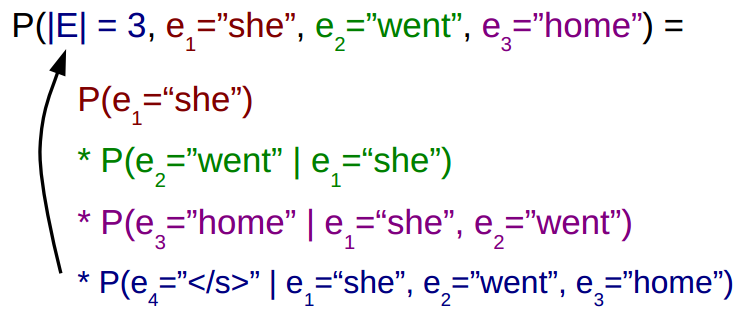
\includegraphics[width=0.6\textwidth]{fig2.png}
\caption{语言模型概率的按词分解计算示意图}
\label{fig:2}
\end{figure}

为了让这个概率计算问题变得可操作一些,我们常常把一个句子的概率分布重定义为:句子中每个词的概率之乘积。
这样一来,一个联合概率可以通过其中每个元素的概率乘起来来计算得出,例如联合概率$P(e_1,e_2,e_3)=P(e_1)P(e_2|e_1)P(e_3|e_1,e_2)$。

在图\ref{fig:2}中,给出了用这种方法来计算“she went home”这句话的概率值的过程。
这里,除了句子中真实的词条之外,我们引入了一个\textit{句末符}(“</s>”),用来表征一个句子在此处终结。
从图中可以看出我们是如何一步一步计算这个概率的:我们顺次计算了“she”出现在句首的概率,“went”紧跟在句首的“she”后面的概率,“home”紧跟在上文“she went”之后的概率,以及句末符“</s>”紧跟在“she went home”之后的概率。
更一般地,我们可以用下面这个表达式来表示:
\begin{equation}\label{eq:4}
 P(E) = \prod_{t=1}^{T+1} P(e_t|e_1^{t-1}),
\end{equation}
其中$e_{T+1}=</s>$。
说回到句末符</s>,我们之所以引入该符号,是为了让它来告诉我们一个句子何时终止。
换句话说,通过检查句末符</s>的位置,我们可以来确定原始语言模型联合概率公式\ref{eq:3}中的句子长度$|E|=T$。
就拿刚才的例子来说,当我们发现句子中第4个词是</s>时,我们就知道了这个句子的长度为3。

有了公式\ref{eq:4}中所述的计算表达式,对语言模型建模的问题,就变成了给定前驱词序列$e_1^{t-1}$的情况下计算当前词$e_t$的概率分布$P(e_t|e_1^{t-1})$的问题。
与直接计算整个句子的概率分布相比,这样的建模方式,可操作性更强了,因为我们现在只需要计算句子中词序列的概率分布就可以了。

在接下来的几个小节中,我们将介绍几种方法,来计算这个词序列的概率分布函数。


\subsection{基于统计的$n$-gram语言模型}
计算概率分布的第一种方法很简单:先准备一个训练语料,我们在该语料里对词串进行计数统计,也就是说,我们统计某个特定词串在语料中出现的频次,然后除以其上文在语料中出现的频次。
这个简单的统计计算方法,可以形式化的表述为如下公式,在图\ref{fig:3}中给出了一个实例。
\begin{equation}\label{eq:5}
  P_{ML}(e_t|e_1^{t-1})=\frac{C_{prefix}(e_1^t)}{C_{prefix}(e_1^{t-1})}.
\end{equation}
这里,$C_{prefix}(\cdot)$是该特定的词串在语料中出现在句首的频次。
这个统计方法,我们称之为\textbf{最大似然估计}(MLE,详情见后续内容),这种方法既简单,又能保证得到的概率模型能对训练语料中见过的句子赋予高概率值。

\begin{figure}[H]
\centering
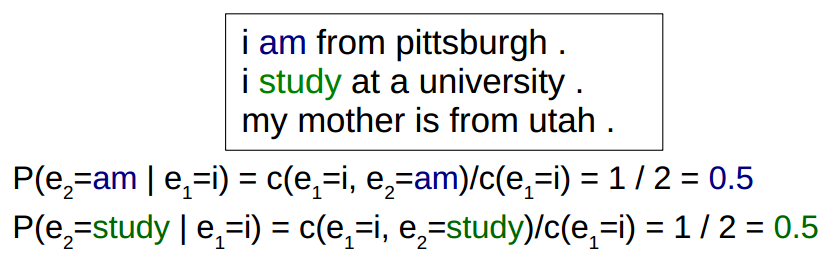
\includegraphics[width=0.6\textwidth]{fig3.png}
\caption{用极大似然估计法计算概率分布的示意图}
\label{fig:3}
\end{figure}

然而,假设有一个我们从未见过的一句话,我们想要用这个模型计算这个句子的概率。
举例来说,在上面例子中的训练语料的基础上,假设我们想要计算“i am from utah .”这句话的概率。
这个句子和我们在训练语料中见过的句子及其相似,但不幸的是,词串“i am from utah”并没有在训练语料里出现过,即$C_{prefix}(i,am,from,utah)=0$,概率值$P(e_4=utah|e_1=i,e_2=am,e_3=from)$就变成零了,因此,通过公式\ref{eq:5}计算得到的这句话的概率值也变成了零。
事实上,这个语言模型,会给所有未在训练语料里出现过的句子,都赋予零概率,也就是说,这个模型失去了对“系统生成的新句子是否是自然的句子”的判断能力,或者说让系统失去了生成新句子的能力,因此,对我们而言,这个简单的模型也就失去了使用价值。

为了解决这个问题,我们采取了两个策略,双管齐下。
第一,我们不再从句首开始计算概率值,而是取一个固定的上文窗口,在计算概率时,只考虑出现在这个窗口范围内的词条,用这种方式来近似的计算真实的概率值。
如果我们将窗口大小限定为$n$,即上文的范围限定为$n-1$个前驱词,那么这个概率值计算公式就近似为
\begin{equation}\label{eq:6}
  P(e_t|e_1^{t-1}) \approx P_{ML}(e_t|e_{t-n+1}^{t-1}).
\end{equation}
基于这个假设的模型,我们称之为\textbf{$n$-gram语言模型}。
具体地,当$n=1$时,我们称之为一元语言模型,当$n=2$时,称之为二元语言模型,$n=3$时,称为三元语言模型,$n \geq 4$时称为四元、五元语言模型,以此类推。

$n$-gram语言模型的参数$\theta$,包含了所有的基于上文$n-1$个词时下一个词出现的概率分布,即:
\begin{equation}\label{eq:7}
  \theta_{t-n+1}^{t} = P(e_t | e_{t-n+1}^{t-1}),
\end{equation}
为了训练一个$n$-gram语言模型,我们需要从训练语料里统计学习这些参数。
简单地,这些参数可以用极大似然估计方法来统计计算得到,计算公式如下:
\begin{equation}\label{eq:8}
  \theta_{t-n+1}^{t} = P_{ML}(e_t | e_{t-n+1}^{t-1}) = \frac{c(e_{t-n+1}^{t})}{c(e_{t-n+1}^{t-1})},
\end{equation}
其中,$c(\cdot)$是词串在语料中任意位置出现的频次。
有时,我们会遇到$e_{t-n+1}$中下标$t-n+1<0$的情况,这种情况下,我们默认$e_{t-n+1}=<s>$,其中<s>是一个特殊的\textit{句首符}。

回到我们前面举的那个例子中,且假设$n=2$,我们可以看到,虽然词串“i am from utah .”在训练语料里并没有出现过,但是,“i am”,“am from”,“from utah”,“utah .”,以及“. </s>”这些词串都在语料里出现过,因此,我们可以将它们的概率值乘起来,来给这个句子计算出一个非零的概率值。

然而,我们还有一个问题:如果遇到训练语料里没有出现过的双词串,我们又该如何处理呢?
碰到这种情况时,这个没有在训练语料里出现过的双词串,其概率值依旧是零,导致我们计算整句概率时也会得到零概率。
$n$-gram语言模型通过对概率值进行\textbf{平滑}来解决这个问题,即在计算$n$元概率时,同时考虑1到$n$元极大似然估计值。
具体地,我们来看看对一元和二元概率的平滑情况,我们假设一个模型会以如下的形式来计算概率值:
\begin{equation}\label{eq:9}
 P(e_t|e_{t-n+1}^{t-1}) = (1 - \alpha)P_{ML}(e_t|e_{t-1}) + \alpha P_{ML}(e_t),
\end{equation}
其中,$\alpha$是一个权值参数,用来控制我们给一元概率分配的权重大小。
只要我们取$\alpha > 0$,不管上文如何,词表中的所有词条都会被赋予一定的非零概率值。
我们称这种方法为\textbf{概率插值法},这是一种能提高概率模型鲁棒性的标准做法,尤其是对那些低频的长尾词更有效。

如果我们想考虑更长的上文,比如$n=3$,$n=4$,$n=5$,或者更长的上文,我们可以通过如下的形式递归地定义我们的概率插值方法:
\begin{equation}\label{eq:10}
 P(e_t|e_{t-m+1}^{t-1}) = (1 - \alpha_{m})P_{ML}(e_t|e_{t-m+1}^{t-1}) + \alpha_{m}P(e_t|e_{t-m+2}^{t-1}).
\end{equation}
上述公式中,右边第一项是$m$元概率模型的极大似然估计,而第二项,是1元到$m-1$元概率模型的插值结果。

当然,还有很多更加复杂的平滑方法,但它们都超出了本文要讨论的范围,不过,如果对平滑方法感兴趣,可以在\cite{chen1996empirical}里找到有关平滑方法的非常棒的总结。

\begin{enumerate}
\item[] \textbf{上下文相关平滑系数}:和上面所述的使用固定的权重系数$\alpha$的做法不同,我们可以改用和上文相关的插值权重系数:$\alpha_{t-m+1}^{t-1}$。这样一来,当有足够数目的训练样本来准确地学习到某个高阶$n$元概率参数时,概率模型将给这个高阶的$n$元概率赋予更大的权值;当训练数据样本很少时,才回退到低阶$n$元概率上来。这个上下文相关的平滑系数,可以通过启发式方法来设定\cite{witten1991zero},或者可以从训练数据中学习得到\cite{neubig2016generalizing}。
\item[] \textbf{回退模型}:在公式\ref{eq:9}中,我们对词表$V$上的两个概率分布进行了插值。而\textbf{回退模型}与其不同,只有当高阶$n$元概率值为零时,才回退到用低阶概率分布来计算词串的概率值。和插值方法相比,回退模型的表达能力更强,也更复杂,论文\cite{goodman2001bit}指出,这两种方法得到的模型效果也是差不多的\cite{goodman2001bit}。
\item[] \textbf{修改模型}:使用一种和极大似然概率$P_{ML}$不同的概率分布也是可行的。在计算概率值之前,从计数结果中“扣除”一个固定的常数,这种方法叫做\textbf{discounting}。当然,也可以修改低阶分布的计数值来反映这样一个事实,只有当高阶分布参数没有被训练语料覆盖到时,模型才会降阶到低阶分布上来。
\end{enumerate}
目前,\textbf{Modified Kneser-Ney平滑}(MKN;\cite{chen1996empirical}),是$n$-gram语言模型常用的、标准的且有效的平滑方法。
MKN平滑同时使用了上下文有关平滑系数、discounting法、以及修改版的低阶概率分布,来确保概率估计的精确性。

\subsection{语言模型的评价方式}
当我们训练得到了一个语言模型之后,下一个问题就是要对这个模型进行测试,来看看它是否能达到如期的效果。
跟很多其他机器学习模型一样,我们评测语言模型时,也需要准备如下三个数据集:
\begin{enumerate}
\item[训练集:] 用来训练模型的参数$\theta$。
\item[开发集:] 用来对不同参数的模型进行选择,或者用来调教模型的\textbf{超参数}。上文所述模型的超参数,包括上文长度$n$以及所使用的平滑方法。
\item[测试集:] 用来评价最终训练所得模型的准确率。
\end{enumerate}

对语言模型而言,我们想知道的,无非是该模型是否能对语言进行准确建模,而对这个准确性而言,我们也有很多定义方法。
最直观的准确性定义,是开发集或测试集上模型的\textbf{似然}。
参数$\theta$在这些数据集上的似然,等价于该参数下模型赋予这些数据的概率值。
比如,我们有一个测试集$\xi_{test}$,这个概率值就是:
\begin{equation}\label{eq:11}
 P(\xi_{test};\theta).
\end{equation}
我们一般会进行这样的假设:这个数据中包含的句子或文档$E$之间是相互独立的,基于这个假设,我们就可以得到:
\begin{equation}\label{eq:12}
 P(\xi_{test};\theta) = \prod_{E \in \xi_{test}} P(E;\theta).
\end{equation}

另一个常用的评价方法,是使用\textbf{对数似然}
\begin{equation}\label{eq:13}
 \log P(\xi_{test};\theta) = \sum_{E \in \xi_{test}} \log P(E;\theta).
\end{equation}
使用对数似然有这么几个方面的原因。
首先,语言模型赋予任何一个句子的概率值,都可能是一个极小的数值,这些极小的概率值乘起来,就会变得无限小,很容易导致浮点数精度溢出问题。
其次,在数学上,通常在对数空间进行相关运算会更方便。比如,在使用基于梯度下降的方法来优化参数时(将在下一节介绍),对求和公式\ref{eq:13}中的参数求偏导数,比对求积公式\ref{eq:12}中的参数求偏导数要来的容易一些。

通常,我们还需要对这个对数似然值进行归一化,即对其除以测试语料中出现的词数:
\begin{equation}\label{eq:14}
 length(\xi_{test}) = \sum_{E \in \xi_{test}} |E|.
\end{equation}
这样一来,我们就能更方便的比较(和对比)模型在不同大小的语料上的评测结果了。

最终,我们得到了评价一个语言模型精确度的最常用指标:\textbf{困惑度},即每个词的平均负对数似然的指数:
\begin{equation}\label{eq:15}
 ppl(\xi_{test};\theta) = e^{-(\log P(\xi_{test};\theta))/length(\xi_{test})}.
\end{equation}
那么,如何直观的理解困惑度这个定义呢?一个直观的解释是:“模型对自己的决策有多困惑?”
更准确的讲,困惑度想表达的是这样一个值:“在生成一个句子中某个位置的词时,如果我们基于语言模型计算的词表概率分布随机的挑选某个词来填这个空,我们平均需要挑选多少次,才能得到那个正确的词?”
我们之所以在研究论文里经常看到用困惑度来评判语言模型的好坏,是因为困惑度计算出来的数值一般都比较大,能让人肉眼就能区分出不同模型之间的好坏差别。

\subsection{未登录词问题}
最后,还有一件重要的事情需要牢记,那就是评测集$\xi_{test}$中出现的某些词,可能在训练集$\xi_{train}$里从未出现过。
我们将这些模型在训练过程中没有“见过”词称为\textbf{未登录词},在测试或使用语言模型时,这些未登录词会给我们带来一些问题,我们必须用某种方法来解决这些问题。
总结起来,语言模型中常见的处理未登录词的方法如下:
\begin{enumerate}
\item[] \textbf{假设词典是封闭集}:有时候,我们可以假设测试集里不会有新词。例如,当我们计算ASCII字符上的语言模型时,认为所有的字符都在训练集里见过这个假设是比较合理的。近似的,在一些语音识别系统中,通常都会简单地给那些未在训练数据里出现过的词赋予零概率,意思就是系统不会对这些词进行识别。
\item[] \textbf{与未登录词分布插值}:如公式\ref{eq:10}所述,我们可以对高阶和低阶分布进行插值。在遇到未登录词时,我们可以认为这是“0”阶分布,可以将1-gram概率定义为一元概率分布和未登录词分布的插值\begin{equation}\label{eq:16} P(e_t) = (1 - \alpha_1)P_{ML}(e_t) + \alpha_1 P_{unk}(e_t).\end{equation}这里,$P_{unk}$是一个概率分布,且为所有的词$V_{all}$都赋予一个概率值,而不只是针对训练语料里学到的词表$V$。具体而言,可以这么操作,训练一个字符级语言模型,能够“拼写”出不在我们词表中的未登录词。或者,我们可以大概估计一下我们所进行建模的语言的词表大小$|V_{all}|$,其中$|V_{all}| > |V|$,并将$P_{unk}$定义为全部词表上的一个均匀分布:$P_{unk}(e_t) = 1 / {V_{all}}$。
\item[] \textbf{添加<unk>符号}:作为最后一种处理未登录词问题的方法,我们可以将训练集$\xi_{train}$里的某些词条删去,将其替换为表示未登录词的特殊符号<unk>。一种常见的做法,是将训练集中只出现了一次的\textbf{单次词}替换掉。通过这种方法,我们可以具体地预测出在何种上文下我们可能会遇到未登录词,而不是用上面讲的插值法来预测具体的某个词。即使我们只是预测了<unk>符,我们也需要估计此处出现的具体的词的概率值,因此,每当在句中位置$i$处预测了<unk>,我们都需要乘上一个概率值$P_{unk}(e_t)$。
\end{enumerate}

\subsection{扩展阅读}
如果想阅读$n$-gram语言模型相关的具体文献,论文\cite{goodman2001bit}将是你的不二之选。
我们上面介绍的简化版$n$-gram语言模型具有很多不足之处,在这篇论文中,作者给出了解决这些不足的一系列方法,并且其介绍过程非常易于理解。

还有一些有关$n$-gram概率模型的扩展问题,有兴趣的读者可以关注:
\begin{enumerate}
\item[] \textbf{大规模语言模型}:语言模型是很多商业工具的组成部件,这些工具中的语言模型,常常是在大规模的网页文本数据上训练而来的。为了处理这种海量的数据集,也有一些高效的数据结构方面的研究\cite{heafield2011kenlm,pauls2011faster},如分布式参数服务器\cite{brants2007large},以及有损压缩算法\cite{talbot2008randomized}等。
\item[] \textbf{语言模型自适应}:在很多情况下,我们需要针对某个具体的用户、或者某个具体的领域,单独训练一个语言模型。自适应技术的做法,是先训练一个大而普适的语言模型,然后再让这个普适模型去自动适应具体的目标使用场景\cite{bellegarda2004statistical}。
\item[] \textbf{基于统计的远距离语言模型}:如上所述,$n$-gram语言模型将上文长度限定为$n-1$,但是在现实中,会有一些词会依赖于句子中很远的某个上文词,或者依赖于整篇文本前面的某些内容。我们在第六节将介绍的循环神经网络语言模型就是用来解决这种远距离依赖问题的,但也有一些非神经网络模型试图去解决这个问题,比如缓存语言模型\cite{kuhn1990cache},主题模型\cite{blei2003latent},skip-gram模型\cite{goodman2001bit}。
\item[] \textbf{句法语言模型}:还有一些模型使用了目标句子的句法信息。例如,我们不仅可以基于句子中相邻的几个词来计算下一个词出现的条件概率分布,我们还可以基于句法上“相邻”的几个词来计算这个条件概率分布\cite{shen2008new}。
\end{enumerate}

%\subsection{练习}

\newpage

\section{对数线性语言模型}
在本节内容中,我们将讨论另一种类型的语言模型:\textbf{对数线性语言模型}\cite{rosenfeld1996maximum,chen2000survey},和上文介绍的基于统计的$n$-gram模型相比,对数线性语言模型另辟蹊径,使用了截然不同的建模方法。

\subsection{形式化定义}
对数线性语言模型和$n$-gram语言模型一样,也是计算给定上文$e_{t-n+1}^{t-1}$时一个特定的词$e_t$出现的概率分布。
然而,对数线性语言模型计算这个概率分布所用的方法,和基于统计的语言模型相比,有很大的不同。
对数线性语言模型计算这个概率值的过程,可以粗略地分为如下几步进行。

\textbf{计算特征值}:对数线性模型的一个基本概念就是\textbf{特征}。简单来讲,特征就是“上文中对预测下一个词有用的信息”。
形式化地,我们可以这样定义一个特征函数$\phi (e_{t-n+1}^{t-1})$,这个函数把上文当做输入,然后输出一个实值\textbf{特征向量$x$}$\in \mathbb{R}^N$,用来描述这个上文的$N$个不同维度特征。

拿我们上一节中介绍的二元语言模型来举例,我们知道“前一个词的编码”这个信息对预测下一个词很有用。
如果我们要用一个实值向量来表示这个信息“前一个词的编码”,我们可以假设词表$V$中的每一个词都有一个与之对应的编号$j$,$1 \leq j \leq |V|$。
然后,我们定义一个特征函数$\phi (e_{t-n+1}^t)$,让其返回一个特征向量$\textbf{x} = \mathbb{R}^{|V|}$,如果$e_{t-1}=j$,就将这个特征向量中第$j$个元素设为1,而其余的元素都设为0。
这种向量,一般被称作\textbf{单极向量\footnote{one-hot vector}},或者\textbf{向量表示},在图\ref{fig:4}(a)中给出了一个样例。
为了后续表述方便,我们也定义了一个函数$onehot(i)$来返回一个“只有第$i$个元素为1而其余元素均为0”的向量。

\begin{figure}[H]
\centering
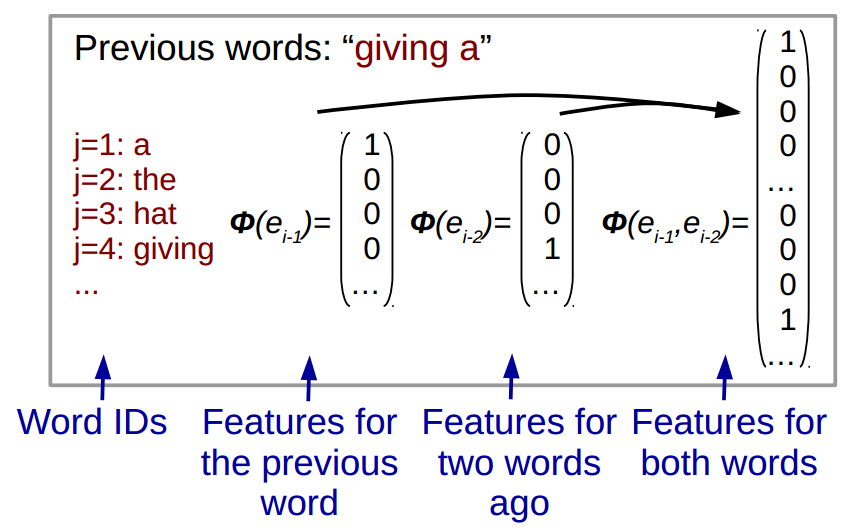
\includegraphics[width=0.6\textwidth]{fig4.png}
\caption{一个上文序列的特征值样例}
\label{fig:4}
\end{figure}

当然,我们没有必要受限于只考虑一个上文词。我们也可以分别计算出$e_{t-1}$和$e_{t-2}$的向量表示,然后将它们首尾拼接起来,就构建出了一个同时考虑了两个上文词的模型。
事实上,我们还能想到更多其他种类的特征函数(将在4.4小节介绍),而能够对多种不同特征弹性驾驭能力,是对数线性语言模型相对于标准的$n$-gram语言模型的一大优势所在。

\textbf{计算得分向量}:一旦我们有了特征向量,我们就可以用这些特征值来预测输出词表$V$的概率分布。
为了达到这个目的,我们先计算出一个得分向量$s \in \mathbb{R}^{|V|}$,其中,每一维数值对应着词表中一个词的似然值,得分越大的词出现的概率也越大。
我们的模型参数$\theta$具体来说就有两个:一个是\textbf{偏置向量}$\textbf{b} \in \mathbb{R}^{|V|}$,用来表征词表中的一个词大体上的似然值,还有一个是\textbf{权值矩阵}$\textbf{W} = \mathbb{R}^{|V| \times N}$,用来表征特征值和得分结果之间的关系。
至此,用来计算某个上文的得分向量的公式定义如下:
\begin{equation}\label{eq:17}
 \textbf{s} = \textbf{Wx} + \textbf{b}.
\end{equation}

值得一提的是,我们要处理的,经常是单极向量或者其他的\textit{稀疏向量},他们都有一个共同的特点,就是其大部分元素为0,仅有个别元素不为0。
因此,我们也可以把公式\ref{eq:17}看成是另一种等价的形式,这样能让计算过程的效率更高。
具体来说,我们不再用一个特别大的特征向量和特别大的权值矩阵相乘,我们可以像下面这样,将权值矩阵中所有被特征向量\textit{激活}的列相加:
\begin{equation}\label{eq:18}
 \textbf{s} = \sum_{\{j:x_j \neq 0\}} W_{\cdot,j}x_{j} + \textbf{b},
\end{equation}
其中,$W_{\cdot,j}$是权值矩阵$W$的第$j$列。
这样一来,可以把计算得分的过程理解为“在权值矩阵中查询特征向量中激活元素所对应的列向量,然后将它们加和”,而不把这个过程看做是矩阵和向量之间的乘法运算。
图\ref{fig:5}中给出了一个例子,就是用这种方式来处理两个特征函数的情况(一个是前一个词,另一个是前一个词前面那个词)。

\begin{figure}[H]
\centering
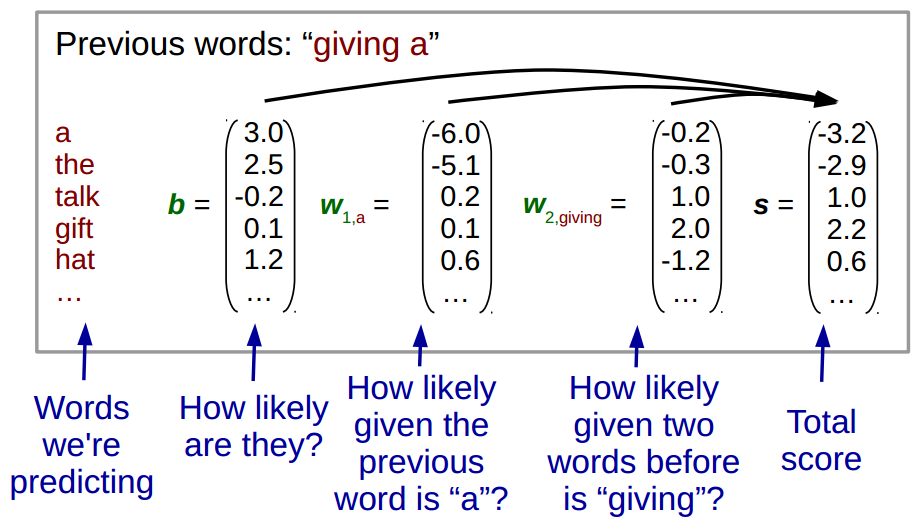
\includegraphics[width=0.6\textwidth]{fig5.png}
\caption{对数线性模型对一个特定上文的得分向量计算过程示意图}
\label{fig:5}
\end{figure}

\textbf{计算概率分布}:值得一提的是,得分向量\textbf{$s$}是一组实数,而不是概率值,这些实数可以为负数或者是大于1的数,而且也没有加和必须为1的限制。
因此,我们需要让这组实数通过这样一个函数来进行如下变形:
\begin{equation}\label{eq:19}
 p_{j} = \frac{exp(sj)}{\sum_{\bar{j}}}exp(s\bar{j}).
\end{equation}
通过计算指数,然后除以词表中所有词对应得分值的指数的加和,就把这些得分值变成一个概率分布了,即满足了在0到1之间且加和为1的限制。

上面这个函数被称为\textbf{softmax函数},一般以下面的向量形式来表示:
\begin{equation}\label{eq:20}
 \textbf{p} = softmax(\textbf{s}).
\end{equation}
用这个函数来处理在上一节中计算得到的得分向量,我们就得到了一种从特征向量出发得到语言模型概率分布的计算方法。

\subsection{学习模型参数}
现在,只剩下最后一个问题了,那就是如何获取并学习参数$\theta$的值,包括权值矩阵$W$和偏置向量$b$。
简单来说,我们所使用的方法,就是迭代地寻找更符合训练语料的参数值。

为了达到优化参数的目的,我们使用机器学习领域里的标准方法。
首先,我们定义一个\textbf{损失函数}$\mathcal{L}(\cdot)$,用来衡量我们的模型在训练语料上表现的不好的程度。
在大多数情况下,我们都用训练语料在给定模型时的\textbf{负对数似然}来定义这个损失值:
\begin{equation}\label{eq:21}
 \mathcal{L}( \xi_{train},\theta ) = - \log P(\xi_{train} | \theta ) = - \sum_{E \in \xi_{train}} \log P(E |\theta).
\end{equation}
假设我们也可以定义如下基于词为粒度的损失函数:
\begin{equation}\label{eq:22}
 \mathcal{L}(e_{t-n+1}^{t},\theta) = \log P(e_t | e_{t-n+1}^{t-1}).
\end{equation}

有了损失函数的定义,剩下的问题,就是我们需要通过优化参数来降低这个损失。
关于优化模型参数,有很多方法,在最近几年,一个较常用的方法是\textbf{随机梯度下降法(SGD\footnote{Stochastic Gradient Descent})}。
随机梯度下降法是一种迭代地优化参数的方法,我们随机的选择一个单词$e_t$(或者mini-batch,将在第5节进行介绍),然后来提升$e_t$的似然。
为了达到这个目的,我们先对损失函数的参数$\theta$中的每个特征参数计算偏导数(梯度):
\begin{equation}\label{eq:23}
 \frac{d\mathcal{L}(e_{t-n+1}^{t},\theta)}{d\theta}.
\end{equation}
然后,我们可以基于这个梯度信息,往降低目标函数损失值的方向迈出一小步:
\begin{equation}\label{eq:24}
 \theta \leftarrow \theta - \eta \frac{d\mathcal{L}(e_{t-n+1}^{t},\theta)}{d\theta}.
\end{equation}
这里的$\eta$是我们的\textbf{学习率}(或者叫做\textbf{步长}),它会决定每次参数更新时更新幅度的大小。
如此,我们就找到了模型的一组新参数,这组新参数能够降低模型在训练数据上的损失,或者说能够提升训练数据的似然。

这个简易版的随机梯度下降方法,不仅简单,而且,它也是可以用来学习大规模系统参数的有效方法之一。
当然,为了让模型训练过程保持稳定,还有一些需要考虑的问题。
\begin{enumerate}
\item[] \textbf{调整学习率}:随机梯度下降方法要求选取$\eta$时格外小心:如果$\eta$过大,训练过程会很不稳定,而且会发散;如果$\eta$过小,训练过程会非常缓慢,而且容易落到不好的局部最优中出不来。\textbf{学习率衰减}是解决这个问题的方法之一,在训练开始时使用较大的学习率,随着学习的进程不断减小学习率,直到训练结束。下文中,我们还会简单介绍一些更复杂的其他方法。
\item[] \textbf{提前停止}:我们知道,我们在训练时普遍会选择一个开发集,来评测模型在这个数据集上的似然,当模型在开发集上达到最优似然值时保存模型并停止训练。这样做,可以有效防止模型过拟合于训练数据而失去泛化能力。另一种防止过拟合和保持训练过程平滑收敛的方法是这样的,在开发集上评测对数似然,当这个对数似然不再提升或者开始变差,就降低学习率。
\item[] \textbf{乱序学习}:随机梯度下降方法在处理训练数据时的一个显著特点,就是每次训练都使用一个样本。因为简单和有效,这样做其实是很好的,但这样做也会产生一些副作用,尤其是当训练样本的排序有一定的偏置的时候。例如,如果我们的训练数据是新闻语料,而且开始部分是时政新闻、然后是体育新闻,再然后是娱乐新闻,这样的顺序,很有可能在训练过程的后段,我们的模型会遇到几百甚至几千条连续的娱乐新闻样本,从而导致参数将偏向一个更偏爱娱乐新闻样本的特征空间。为了防止这个问题,通常(在此强烈推荐)在每一轮训练模型参数之前,都要随机的打乱训练样本的出现顺序。
\end{enumerate}

当然,机器学习研究者还提出了一些其他参数更新方法,同样可以达到使训练过程更稳定和有效的目的。
下面列举了一些具有代表性的方法:
\begin{enumerate}
\item[] \textbf{惯性随机梯度下降\cite{holyoak1987parallel}}:与每次在当前梯度方向上走一小步的过程不同,惯性随机梯度下降方法所使用的梯度是历史上所有梯度的平均值。这样一来,可以减轻简单的随机梯度下降方法的“抖动”倾向,让参数优化的过程能够更加地平滑。
\item[] \textbf{AdaGrad\cite{duchi2011adaptive}}:AdaGrad关注于这样一个事实:一些参数的更新频率比其他参数的要高很多。例如,在上面的模型中,上文中出现的低频词所对应的权值矩阵中的列向量,在训练过程中只会被更新几次而已,而偏置向量$\textbf{b}$会在每一个训练样本上都进行更新。基于此事实,AdaGrad会对每一个参数具体地动态调整学习率$\eta$的值,频繁更新的参数,如偏置向量$\textbf{b}$,每次会进行很小幅度的更新,而不频繁更新的参数,如权值矩阵$W$,则每次做较大幅度的更新。
\item[] \textbf{Adam\cite{kingma2014adam}}:Adam也是一种为每一个参数单独计算学习率的方法。通过记录每个参数的历史梯度的平均值和方差,使用类似于前面两种方法来计算梯度。由于能显著加快很多数据集上的模型训练收敛速度,缩短了实验迭代的周期,因此Adam方法成为了时下最受欢迎的优化方法之一。然而,该方法也有自身的缺点,那就是趋向于过拟合,因此,如果对模型效果有较高的要求,那么相较于标准的随机梯度下降方法而言,在使用Adam方法时需要更加小心谨慎才行。
\end{enumerate}
再论文\cite{ruder2016overview}中,作者对这几个不同的参数优化方法做了一个很好的综述,提供了很多公式和说明,并指出了使用随机优化参数方法时的一些注意事项。

\subsection{对数线性模型的偏导数}
现在,只剩下最后一个问题,那就是如何计算损失函数中每个参数的偏导数了。
为此,我们先从头到尾梳理一下损失函数的计算过程:
\begin{eqnarray}
 \textbf{x} & = & \phi (e_{t-m+1}^{t-1}) \label{eq:25} \\
 \textbf{s} & = & \sum_{j:x_j \neq 0} W_{\cdot,j}x_j + \textbf{b} \label{eq:26} \\
 \textbf{p} & = & softmax(\textbf{s}) \label{eq:27} \\
 \mathcal{L} & = & - \log \textbf{p}_{e_t} \label{eq:28}
\end{eqnarray}
如此一来,可以用链式法则来计算
\begin{eqnarray}
 \frac{d\mathcal{L}(e_{t-n+1}^t,W,b)}{d\textbf{b}} & = & \frac{d\mathcal{L}}{d\textbf{p}}\frac{d\textbf{p}}{d\textbf{s}}\frac{d\textbf{s}}{d\textbf{b}} \label{eq:29} \\
 \frac{d\mathcal{L}(e_{t-n+1}^t,W,b)}{d\textbf{W}_{\cdot,j}} & = & \frac{d\mathcal{L}}{d\textbf{p}}\frac{d\textbf{p}}{d\textbf{s}}\frac{d\textbf{s}}{d\textbf{W}_{\cdot,j}} \label{eq:30}
\end{eqnarray}
我们可以发现,损失函数对偏置向量和权值矩阵的每一列的偏导数为:
\begin{eqnarray}
 \frac{d\mathcal{L}(e_{t-n+1}^t,W,b)}{d\textbf{b}} & = & \textbf{p} - onehot(e_t) \label{eq:31} \\
 \frac{d\mathcal{L}(e_{t-n+1}^t,W,b)}{d\textbf{W}_{\cdot,j}} & = & x_j (\textbf{p} - onehot(e_t)) \label{eq:32}
\end{eqnarray}
验证这些公式的准确性的工作,就留给读者自己完成了。提示:在计算偏导数时,相比于直接操作$\textbf{p}$来说,操作$\log \textbf{p}$会更容易一些。

\subsection{语言模型的其他特征}
对数线性模型之所以好,是因为该模型能让我们更灵活的设计特征,只要我们觉得这些特征对预测下一个词有用,我们就可以很方便的将这个特征放进模型中去。
例如,这样的特征包括但不限于:
\begin{enumerate}
\item[] \textbf{上文词特征}:如上例所示,我们可以用$e_{t-1}$或者$e_{t-2}$的编码作为上文词特征。
\item[] \textbf{上文词类特征}:上文中的词可以按相互之间的相似度归到不同的词类中(使用布朗聚类方法\cite{brown1992class}),与其用单极向量来表示每个特定的词,我们可以用单极向量来表示每个词所属的词类\cite{chen2009shrinking}。如此一来,同一个类中的词条可以共享此类的统计信息,从而使模型具有了更好的泛化能力。
\item[] \textbf{上文后缀特征}:也许我们想要这样一个特征函数,每当前一个词以“...ing”结尾或其他类似的后缀结尾时,这个特征函数就会被激活。这样,模型能够学到更加泛化的构词法相关的特征,比如哪些词倾向于出现在正在进行时态动词的后面等。
\item[] \textbf{词袋子特征}:我们也可以用所有在句子上文窗口中出现的词作为特征,而不是只用前$n$个词。这相当于计算前一个句子中的每一个词的单极向量,然后将它们加起来,而不是拼接在一起。这种做法,会损失掉词条所在的句中位置信息,但能够捕获“哪些词倾向于在同一个句子或同一个文档中共现”的信息。
\end{enumerate}

当然,同时使用不同的特征之间的组合信息也是完全可行的(例如,将词与词的组合信息作为上文特征等)。
这是构造更具解释性的特征集的方法之一,当然也有其不足之处,最明显的短板,就是这样做会无限的扩大特征空间的范围。
我们在第5.1小节讨论这些组合特征的具体使用方法。

\subsection{扩展阅读}
本节所介绍的语言模型,基本可以理解为$n$-gram语言模型的特征化版本。
当然,还有不少其他的线性特征化模型,包括:
\begin{enumerate}
\item[] \textbf{整句语言模型}:这些模型预测整句话的概率分布然后以整句为单位进行概率归一化\cite{rosenfeld2001whole},而不是一个词一个词的进行预测。可以通过引入一些其他特征来达到这个目的,比如句子长度的概率分布信息,或者诸如“该句子中是否含有动词”这样的特征。
\item[] \textbf{判别语言模型}:如果我们只是希望语言模型能够判别系统输出的一个句子是否是正确的句子,那么,有时候直接按这个目标训练模型会更好,然后用训练得到的模型对系统输出结果进行重排序(re-rank),从而得到更高的准确率\cite{roark2004discriminative}。即便训练时我们没有真实的(人工标注过的)反例样本,我们也可以通过“伪造”反例样本的方法来进行模型训练,从而达到训练判别模型参数的目的\cite{tsujiiythu2007discriminative}。
\end{enumerate}

%\subsection{练习}

\newpage

\section{神经网络和前馈神经网络语言模型}
在这一节,我们将介绍基于\textbf{神经网络}的语言模型,一种学习更加复杂的函数的方法,不仅提高了概率分布的预测准确率,而且减少了人工特征工程的烦恼。

\subsection{特征组合的潜力与问题}
在介绍神经网络的具体技术细节之前,我们先来看看图\ref{fig:6}中的一个直观例子。
在这个例子中,我们可以看到$e_{t-1}$=“farmers”和$e_t$=“hay”是可搭配的(在句子“farmers grow hay”中),而$e_{t-1}$=“eat”也与之可搭配(在句子“cows eat hay”中)。
如果我们使用的对数线性模型中,有一个特征集与$e_{t-1}$相关,而另一个特征集与$e_{t-2}$相关,任何一个特征集都不能把“farmers eat hay”这个不自然的短语区分出来。

\begin{figure}[H]
\centering
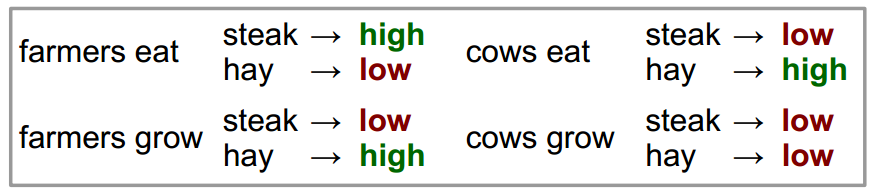
\includegraphics[width=0.6\textwidth]{fig6.png}
\caption{多个词的组合会对下一个词的概率分布的影响示意图}
\label{fig:6}
\end{figure}

我们可以通过下面这种方法来解决这个问题,即另取一个特征集,来学习每两个词对“$e_{t-2},e_{t-1}$”的向量表示。
这样一来,上文词对特征$e_{t-2}$=“farmers”,$e_{t-1}$=“eat”的向量对于“hay”会赋予一个低得分,从而解决这个问题。
然而,加入这种组合特征有一个重要缺陷:这样做会极大的扩大参数个数,我们不仅需要为每一个词对“$e_{i-1},e_i$”设置$O(|V|^2)$个参数变量(用于二元组合特征表示),还需要对任意三元组“$e_{i-2},e_{i-1},e_i$”设置$O(|V|^3)$个参数变量(用于三元组合特征表示)。
不难看出,这会让模型占用的内存空间急剧扩大,且如果没有足够的训练样本数据,这些参数也无法学的很到位。

由于这种组合特征很重要,但又很难学习到,所以,研究人员提出了一系列方法来使用这些特征,比如\textbf{有核支持向量机\footnote{Kernelized Support Vector Machines}}\cite{cortes1995support}和\textbf{神经网络}\cite{rumelhart1988learning,goldberg2016primer}。
具体到本节的内容,我们将介绍神经网络模型,这个模型相对而言更加灵活,且容易在大数据上进行参数训练,也是介绍端到端模型之前需要掌握的最基础内容。

\subsection{神经网络模型概述}
为了理解神经网络模型的具体细节,我们先来举个学习一个函数的例子,这个函数我们无法用前一节介绍的简单线性分类器来学到,这个函数的具体表达为:接收输入$\textbf{x} \in \{-1,1\}^2$,然后当$x_1=x_2$时输出$y=1$,否则输出$y=-1$。
这个函数对应的函数图像如图\ref{fig:7}所示。

\begin{figure}[H]
\centering
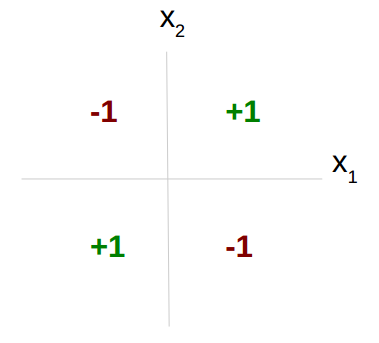
\includegraphics[width=0.3\textwidth]{fig7.png}
\caption{一个线性不可分的方程}
\label{fig:7}
\end{figure}

我们尝试解这个方程的第一步,是定义如下的线性模型来解这个问题:
\begin{equation}\label{eq:33}
 y = W\textbf{x} + b.
\end{equation}
然而,这类线性方程还没有足够的能力来解决手头的问题。

因此,我们转而使用稍加复杂一些的非线性方程,形式化的定义如下:
\begin{eqnarray}
 \textbf{h} & = & step(W_{xh}\textbf{x} + \textbf{b}_h) \nonumber \\
 y & = & \textbf{w}_{hy}\textbf{h} + b_y. \label{eq:34}
\end{eqnarray}
计算过程分两步进行:第一步,计算\textbf{隐层},这一步将输入$\textbf{x}$转换成一个隐层向量$\textbf{h}$;第二步,计算\textbf{输出层},这一步根据隐层向量$\textbf{h}$计算出最终的结果$y$。
两层节点都包括使用权值矩阵$W$和偏置向量$\textbf{b}$的\textbf{线性变换}操作,然后紧跟一个非线性的$step(\cdot)$函数,这个函数定义如下:
\begin{equation}\label{eq:35}
 step(x) = \left\{ \begin{array}{ll}
  1 & \textrm{if $x > 0$} \\
  -1 & \textrm{otherwise}
  \end{array} \right. 
\end{equation}
这个函数是被称为\textbf{多层感知机\footnote{Multi-layer Perceptrons}}的一类神经网络的一个特例。
宽泛地讲,多层感知机包含一个或多个隐层,每个隐层先进行线性变换然后再进行非线性化操作(例如这里使用的step函数),最终到达输出层,计算出不同的输出结果。

\begin{figure}[H]
\centering
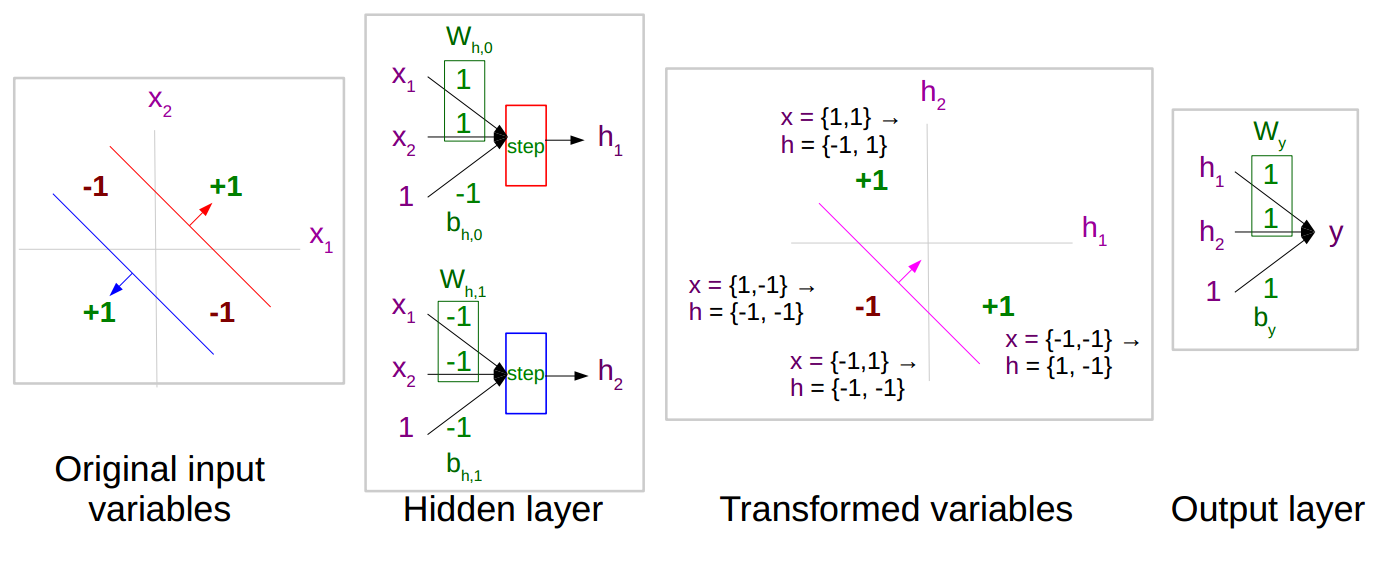
\includegraphics[width=1\textwidth]{fig8.png}
\caption{用一个简单的神经网络来表示图\ref{fig:7}中的非线性方程}
\label{fig:8}
\end{figure}

图\ref{fig:8}展示了这种网络之所以能够很好的处理图\ref{fig:7}所示的非线性分类问题的原因。
简单说来,我们可以看到,第一个隐层将原始输入$\textbf{x}$\textit{映射}到另一个特征空间里的隐层向量$\textbf{h}$,在原空间不可分类的问题在这个新的特征空间就变得线性可分了。
具体到这个例子中,我们可以看到,$\textbf{h}$现在处在一个线性可分空间中,使得我们可以在这个空间中定义一个线性分类函数(使用$w_y$和$b_y$)就可以准确的计算出我们想要的输出值$y$。

如上所述,多层感知机是神经网络的一个具体形式。
更广泛地说,神经网络可以被理解为一个链式函数序列(如上面所说的线性变换和step函数,当然也包括很多其他的函数),在给定输入的情况下计算得到想要的输出值。

神经网络模型之所以强大,是因为这样一个事实,通过用链式计算的方法将一系列简单的方程连在一起,就可以表达出更加复杂的函数,而且这个复杂的函数容易进行训练,并且模型参数可以不用那么多。
实际上,上面所介绍的一个简单的单层神经感知机是一个\textbf{通用函数逼近器\footnote{Universal Function Approximator}}\cite{hornik1989multilayer},也就是说,只要其隐层$\textbf{h}$包含足够多的节点,这个模型就能用来拟合任意一个函数,拟合准确率随隐层节点数的不同而不同。

我们将在5.3小节介绍神经网络模型的训练过程,然后在第5.5节,我们介绍神经网络语言模型时会举几个例子,来说明这种模型是如何做到降低参数规模的。

\subsection{训练神经网络}
现在我们有了如公式\ref{eq:34}所示的模型,我们需要训练其参数$W_{mh},b_{h},w_{hy},b_y$。
还记得我们上一节中介绍的梯度下降训练方法吧,我们定义一个损失函数$\mathcal{L}(\cdot)$,然后针对每个模型参数求这个损失函数下的梯度,接着在降低梯度的方向上走一小步来迭代参数。
在这里,我们使用回归问题常用的\textbf{平方误差\footnote{Squared-error Loss}}作为我们的损失函数,这个损失用来衡量系统输出$y$与给定的正确“答案”$y^*$之间的差异大小,其形式化的定义如下:
\begin{equation}\label{eq:36}
 \mathcal{L}(y^*,y) = (y^* - y)^2.
\end{equation}

下一步,我们需要计算各参数的偏导数。
在这里,我们遇到了一个问题:这个$step(\cdot)$函数对求导不太友好,因为其导数形式如下:
\begin{equation}\label{eq:37}
 \frac{\mathnormal{d}step(x)}{\mathnormal{d}x} = \left\{ \begin{array}{ll}
  undefined & \textrm{if $x = 0$} \\
  0 & \textrm{otherwise}
  \end{array} \right. 
\end{equation}
因此,一般都会用其他的非线性函数来代替这个$step(\cdot)$函数,比如双曲正切函数。
正切函数的图像如图\ref{fig:9}所示,形状上看,它更像是step函数的松弛版,但是连续可导的,这一点使其易于通过梯度下降方法来进行训练。
当然,非线性函数还有很多其他的选择,其中最受欢迎的,是整流线性单元(ReLU\footnote{Rectified Linear Unit}):
\begin{equation}\label{eq:38}
 ReLU(x) = \left\{ \begin{array}{ll}
  x & \textrm{if $x > 0$} \\
  0 & \textrm{otherwise}
  \end{array} \right.
\end{equation}
如图\ref{fig:9}中右图所示。
简单来说,正切函数tanh有一个“饱和”问题,即当输入值$x$的绝对值很大($x$是极大的正数或极小的负数)时,其偏导数值会变得非常小,而整流线性单元ReLU解决了这个问题。
包括本节将要介绍的语言模型在内,相关实验结果均表明,ReLU是tanh函数的一个非常有效的替代者\cite{vaswani2013decoding}。

\begin{figure}[H]
\centering
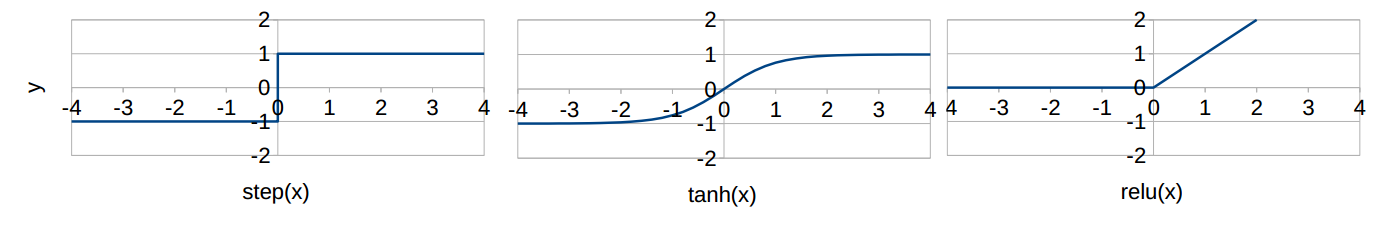
\includegraphics[width=1\textwidth]{fig9.png}
\caption{多种非线性函数示例}
\label{fig:9}
\end{figure}

那么,我们就用非线性激发函数tanh来代替我们的网络中的step函数,现在,我们就可以像在第4.3节所做的那样,开始计算偏导数了。
首先,我们来分步计算损失函数:
\begin{eqnarray}
 \textbf{h}^{'} & = & W_{xh}\textbf{x} + \textbf{b}_h \nonumber \\
 \textbf{h} & = & tanh(\textbf{h}^{'}) \nonumber \\
 y & = & \textbf{w}_{hy} \textbf{h} + b_y \nonumber \\
 \mathcal{L} & = & (y^* - y)^2 \label{eq:39}
\end{eqnarray}
接着,我们再次使用链式规则,来计算每个参数的偏导数:
\begin{eqnarray}
 \frac{d\mathcal{L}}{db_y} & = & \frac{d\mathcal{L}}{dy} \frac{dy}{db_y} \nonumber \\
 \frac{d\mathcal{L}}{d\textbf{w}_{hy}} & = & \frac{d\mathcal{L}}{dy} \frac{dy}{d\textbf{w}_{hy}} \nonumber \\
 \frac{d\mathcal{L}}{d\textbf{b}_h} & = & \frac{d\mathcal{L}}{dy} \frac{dy}{d\textbf{h}} \frac{d\textbf{h}}{d\textbf{h}^{'}} \frac{d\textbf{h}^{'}}{d\textbf{b}_h} \nonumber \\
 \frac{d\mathcal{L}}{dW_{xh}} & = & \frac{d\mathcal{L}}{dy} \frac{dy}{d\textbf{h}} \frac{d\textbf{h}}{d\textbf{h}^{'}} \frac{d\textbf{h}^{'}}{dW_{xh}} \label{eq:40}
\end{eqnarray}

我们可以通过手算的方法,来计算得到模型中所有参数的精确偏导数。
有兴趣的读者完全可以这么做,但即使是上面所述的这种简单模型,这样做也需要相当大的计算和查错处理工作量。
尤其当要处理更加复杂的模型时,比如接下来的章节中将要介绍的模型,更是如此。

\begin{figure}[H]
\centering
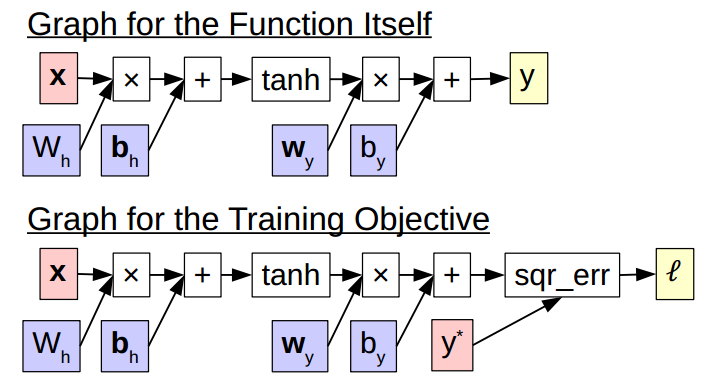
\includegraphics[width=0.5\textwidth]{fig10.png}
\caption{函数本身及其损失函数的计算图}
\label{fig:10}
\end{figure}

幸运的是,当我们在编程实现一个神经网络模型时,有一个非常有用的工具\textbf{自动偏微分\footnote{Automatic Differentiation(autodiff)}}\cite{wengert1964simple,andreas1991dif},可以为我们节省很多额外的工作量。
为了理解自动偏微分法,把公式\ref{eq:39}中的计算过程看做是一个\textbf{计算图}数据结构会很有帮助,在图\ref{fig:10}中给出了两个计算图示例。
在这些图中,一个图结点或者表示这个网络的一个输入,或者表示一个计算过程的结果,计算过程如乘法、加法、双曲正切,或者平方错误差等。
图中的第一个计算图,是一个函数的计算过程,我们在使用这个模型来做预测的时候,会用到这个计算图。而第二个计算图,是计算损失函数的过程,我们在训练时会用到。

自动偏微分,是一个动态规划算法,会在图\ref{fig:10}中第二个计算图上分两步进行操作,这两步操作具体为:
\begin{itemize}
\item \textbf{前向计算过程},按照计算图的拓扑结构来访问每个结点,计算出公式\ref{eq:39}所示的各结点的实际计算结果。
\item \textbf{后向传播过程},按照计算图的拓扑结构逆向访问每个结点,计算出公式\ref{eq:40}所示的各个偏微分。
\end{itemize}
很明显,这样的形式化过程有个好处,根据计算图来计算的函数方程可以相对复杂些,只要这个复杂函数能够通过结合多个简单结点来得到,而这一简单结点可以用来计算函数$f(x)$和其偏微分$f'(x)$,我们就可以用自动偏微分方法,来使用动态规划的计算过程,来得到这个复杂函数中每个参数的偏导数,而不需要徒手计算了。

因此,为了编程实现一个通用的神经网络模型的训练算法,需要先编程实现这两个动态规划过程,包括独立的前向计算过程,和我们所需的每一种结点的后向偏微分结果。
虽然编程实现这两个动态规划算法不是很复杂,但也需要相当的工作量,可喜的是,现在有一批工具包,可以用来做通用的自动偏微分\cite{bendtsen1996fadbad,hogan2014fast},或者是提供了针对机器学习或神经网络专门定制的自动偏微分\cite{abadi2016tensorflow,bergstra2010theano,collobert2002torch,tokui2015chainer,neubig2017dynet}。
这种计算图的数据结构、结点、后向传播、参数最优化算法等等的开源实现,不仅可以用来高效可靠地训练神经网络模型,也降低了研究人员的开发实现难度,从而让他们开始更多的考虑设计自己的新模型,而不是把大把的时间花费在工程实现上。
在下一节中,我们将介绍如何使用一个开源工具包\textbf{DyNet\footnote{http://github.com/clab/dynet}}来实现我们自己的模型,这个开源工具包提供的编程接口,能让我们方便地对将要介绍的端到端模型进行编程实现。

\subsection{一个实现样例}
图\ref{fig:11}中,给出了一个用\textbf{DyNet}工具来实现上述神经网络模型的例子,我们将按行讲解这段代码。
\begin{figure}[H]
\centering
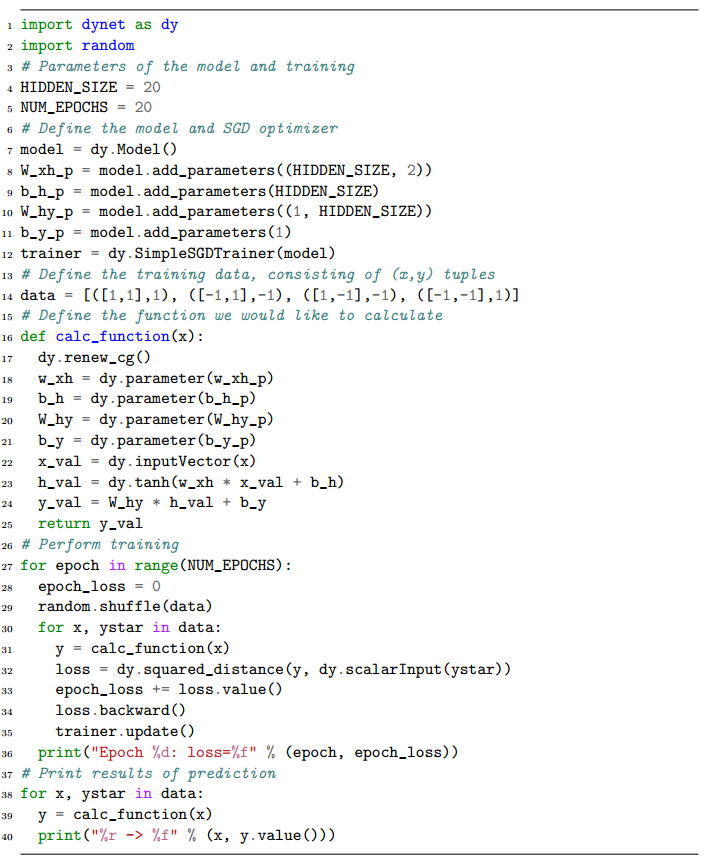
\includegraphics[width=1\textwidth]{fig11.png}
\caption{使用工具DyNet训练一个多层神经感知网络的示例}
\label{fig:11}
\end{figure}
第1-2行,是引用必要的包。
第4-5行,定义了模型的必要参数:隐层向量\textbf{$h$}的大小和训练时所需进行的迭代次数。
第7行,初始化一个DyNet模型,我们将在其中保存所有需要学习的参数。
第8-11行,对参数$W_{xh}$,$b_h$,$w_{hy}$和$b_y$按合适的大小进行初始化,以便能和公式\ref{eq:39}所需的要求相匹配。
第12行,初始化一个“训练器”,它可以按照选定的更新规则来对模型的参数进行更新(这里我们使用了简单的随机梯度下降法,但是使用AdaGrad,Adam或其他优化方法的训练器也是存在的)。
第14行,为训练过程生成数据,这里我们是训练图\ref{fig:7}所示的函数。

第16-25行,定义了一个函数,它的输入是\textbf{$x$},然后生成一个计算图来完成公式\ref{eq:39}的计算过程。
首先,第17行,先生成一个计算某个训练样本的计算图。
第18-21行,把参数以DyNet变量的形式加到计算图中。
第22行,使用Python的list来表示当前的输入,并将其作为DyNet变量加入到计算图中。
第23行,计算隐层向量\textbf{$h$}。
第24行,计算出结果$y$。
第25行,返回这个计算结果。

第27-36行,在训练数据上进行$\mathrm{NUM\_EPOCHS}$次迭代训练。
第28行,定义了一个变量来记录本轮迭代的损失总和,用于本轮迭代后的日志输出。
第29行,对训练数据进行打乱顺序,正如4.2小节中所推荐的那样。
第30-35行,进行随机梯度下降训练过程,顺次使用每一个训练样本进行参数学习。
第31行,计算函数的输出值,第32行,用前一行的的输出值来计算损失函数值。
第33行,执行前向计算过程,来得到损失值并将其加到本轮的损失值总和上。
第34行,执行后向传播过程,第35行,进行参数更新。
在这一轮迭代过程结束后,在第36行打印本轮迭代的损失值,用来观察损失值是否在降低,来检验我们的模型训练过程是否在收敛。

最后,在训练过程结束后,在第38-40行,我们输出最终的计算结果。
在实际情况中,这一步将会在另一个数据集(测试集)上进行。

\subsection{神经网络语言模型}
基础部分到此告一段落,是时候把神经网络模型应用到语言模型\cite{nakamura1990neural,bengio2003neural}中了。
一个前馈神经网络语言模型,和我们在前一节介绍的对数线性语言模型非常相似,两者区别仅仅是在输出层之前多了一个或多个非线性隐层。

首先,我们回顾一下三元对数线性语言模型。
在这个模型中,假设我们有两个特征集合,分别表示了$e_{t-1}$(特征向量表示为$W^{(1)}$)和$e_{t-2}$(特征向量表示为$W^{(2)}$)的特征表示,该对数线性模型的公式如下:
\begin{eqnarray}
 \textbf{s} & = & W_{\cdot,e_{t-1}}^{(1)} + W_{\cdot,e_{t-2}}^{(2)} + \textbf{b} \nonumber \\
 \textbf{p} & = & softmax( \textbf{s} ). \label{eq:41}
\end{eqnarray}
在这里,我们将权值矩阵中相应列向量和偏置向量加起来得到得分向量,再用softmax操作,将得分向量转换为概率分布。

\begin{figure}[H]
\centering
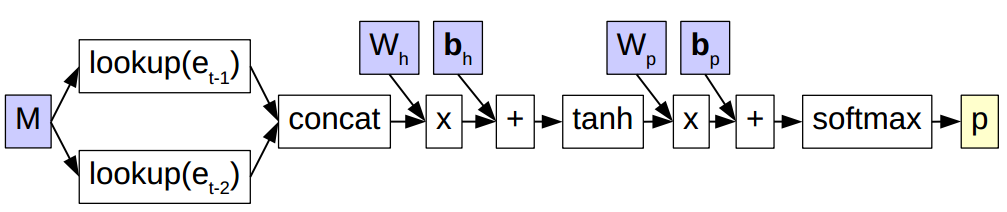
\includegraphics[width=0.8\textwidth]{fig12.png}
\caption{三元前馈神经网络语言模型的计算图示例}
\label{fig:12}
\end{figure}

与此不同,一个单层的三元神经网络语言模型的架构如图\ref{fig:12}所示,我们用如下公式来对其进行描述:
\begin{eqnarray}
 \textbf{m} & = & concat(M_{\cdot,e_{t-2}},M_{\cdot,e_{t-1}}) \nonumber \\
 \textbf{h} & = & tanh( W_{mh}\textbf{m} + \textbf{b}_h) \nonumber \\
 \textbf{s} & = & W_{hs}\textbf{h} + \textbf{b}_s \nonumber \\
 \textbf{p} & = & softmax(\textbf{s}) \label{eq:42}
\end{eqnarray}

在第一行,我们得到了上文$e_{i-n+1}^{i-1}$的向量表示\textbf{m}(作为特例,我们处理三元模型,即$n=3$)。
这里,$M$是一个$|V|$列$L_m$行的矩阵,其中每一列长度为$L_m$的向量为词表中对应的一个词的向量表示。
这个向量叫做\textbf{词嵌入\footnote{Word Embedding}}或\textbf{词表示\footnote{Word Representation}},即词表中对应的某个词的实数向量表示。
用一个实数向量来表示一个词,是一件很有实际意义的事,有用之处在于,向量中的每一维反映了这个词的不同维度的特征。
例如,向量中的某一个维度表示这个词可能是个名词,或者向量中的某个维度用来表示这个词是否是一个动物,或者另一个维度来表示这个词是否可数等。

在图\ref{fig:13}中,我们给出了一个样例程序,教你如何借助DyNet工具包来实现从矩阵中查找一个列向量的方法。

\begin{figure}[H]
\centering
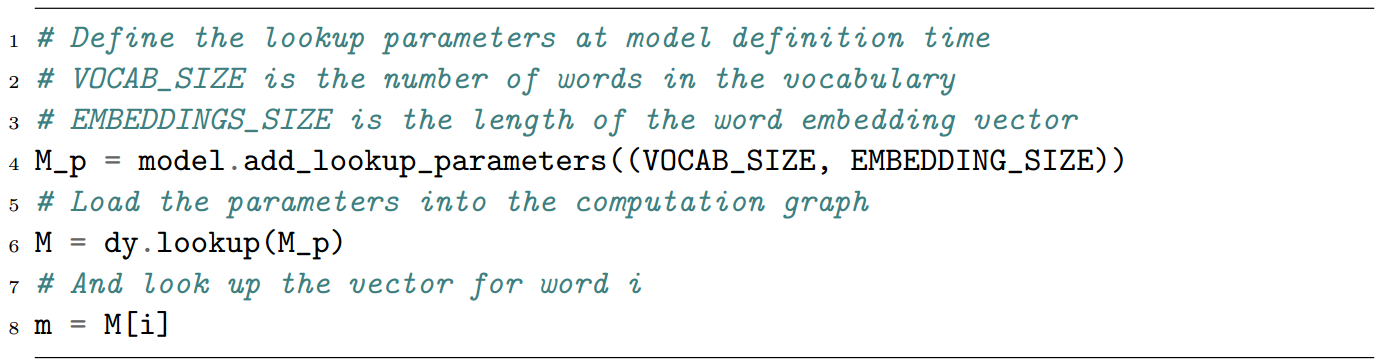
\includegraphics[width=1\textwidth]{fig13.png}
\caption{在DyNet中进行lookup操作的代码样例}
\label{fig:13}
\end{figure}

将上文中出现的所有词的向量首尾相接,就得到了向量$\textbf{m}$,由此可知$|\textbf{m}|=L_m * (n-1)$。
一旦我们有了这个上文特征向量$\textbf{m}$,我们就可以让其通过一个隐层来得到向量$\textbf{h}$。
这样一来,模型可以学习到反映上文信息的多个词之间的组合特征。
这样就使模型的表达能力得到了大大加强,使模型能够表示比图\ref{fig:6}所示更复杂的情况。
例如,给定一个上文“cows eat”,而向量$M_{\cdot,cows}$中的某个元素表示这个词是一个“大型农场动物”(如:“cow”,“horse”,“goat”),而向量$M_{\cdot,eat}$中的某些元素对应了“eat”这个动作和与其相似的其他动作(如“consume”,“chew”,“ingest”)的表示,然后,我们可以学到隐层$\textbf{h}$中的某个节点,当上文表示“农场动物吃的东西”时,这些隐层节点就会被激活。

下一步,我们来计算每个词的得分向量:$\textbf{s} \in \mathbb{R}^{|V|}$。
这个得分向量,可以通过对隐层向量$\textbf{h}$做变换而得到,这个变换过程有自己的一套参数,即权值矩阵$W_{hs} \in \mathbb{R}^{|V| \times |h|}$和偏置向量$\textbf{b}_s \in \mathbb{R}^{|V|}$。
最后,把计算得到的得分向量通过softmax函数,进而得到了概率分布$\textbf{p}$,就像我们在对数线性语言模型中做的那样。
至于训练过程,如果我们知道词$e_t$,我们可以用如下公式计算损失函数,和对数线性模型的做法类似:
\begin{equation}\label{eq:43}
 \mathcal{L} = - \log (p_{e_t}).
\end{equation}
DyNet工具包中有一个很方便的函数,可以在给定得分向量$\textbf{s}$时计算出负对数似然损失值:

\begin{figure}[H]
\centering
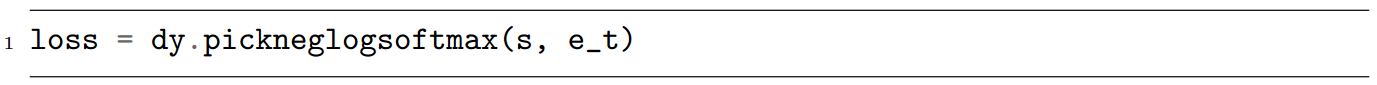
\includegraphics[width=1\textwidth]{fig131.png}
\end{figure}

当我们将神经网络语言模型与第3节中介绍的$n$-gram语言模型做个比较,就不难发现神经网络这种建模方式的好处了,总结起来,有这么三方面的好处:
\begin{enumerate}
\item[] \textbf{更好的上文泛化能力}:$n$-gram语言模型将每个词作为独立的个体对待。通过使用词表示向量$M$,就可以让相似的词聚在一起,并让这些相似词在预测下一个词时具有相似的预测性质。为了达到同样的目的,$n$-gram模型需要额外的训练出一个词类来(基于词类的$n$-gram语言模型),而且要有效使用这个词类信息,并不是一件简单的事情\cite{brown1992class}。
\item[] \textbf{更泛化的上文特征组合能力}:在一个$n$-gram语言模型中,我们需要以参数的形式记录下面两组词\[\{cow,horse,goat\}\times\{consume,chew,ingest\}\]所能组合出的所有情况,来表达上文“农场动物吃的东西”这个意思。这样一来,参数规模和一个词类中词条的个数成指数关系,而在训练数据非常有限的情况下,学习这么大规模的参数是非常困难的。神经网络模型通过学习隐层表示的新思路,将这种近乎无限的组合关系借助有限个参数来进行表示,从而解决了这个参数爆炸问题。
\item[] \textbf{能够跳过前驱词的能力}:$n$-gram语言模型常常从较长的上文(如,“两个上文词$e_{t-2}^{t-1}$”)顺次回退到较短的上文(如,“前一个词$e_{t-1}$”),但这个回退过程不允许“跳过”某个词,比如只考虑目标词和“两个词之前的词$e_{t-2}$”的相关性。对数线性模型和神经网络模型则能够很自然的解决这类远距离依存问题。
\end{enumerate}

\subsection{扩展阅读}
除了上面介绍的方法之外,神经网络语言模型还有很多其他的扩展问题值得探讨。
\begin{enumerate}
\item[] \textbf{Softmax估计}:训练对数线性语言模型或神经网络语言模型时,都会遇到一个问题,在学习每一个训练样本时,都需要计算一个很大的得分向量$\textbf{s}$,然后通过softmax函数来得到相应的概率分布。当词表规模$|V|$变大时,这一过程会变得非常耗时。因此,研究人员提出了很多种降低这部分计算开销的方法。其中的一类方法,是先在词表中采样出一个子集$V' \in V$使得$|V'| << |V|$,然后在这个子集上进行得分计算和损失估计等操作。另一类方法与前一类类似,只是训练目标变成让这个子集中的其他词的模型得分远低于真实目标词$e_t$的模型得分\cite{collobert2011natural},还有一些从概率角度出发的方法,比如\textbf{importance sampling}\cite{bengio2008adaptive}或\textbf{noise-contrastive estimation}(NCE;\cite{mnih2012fast})。有趣的是,对于其他的目标函数如线性回归、特殊的softmax方法\textbf{spherical softmax},可以通过使用不同的目标函数,来让计算目标函数的过程并不与词表大小成正相关\cite{vincent2015efficient},从而避免大词表引起的计算开销问题。
\item[] \textbf{其他Softmax架构}:加快训练速度的另一种技巧,就是创造一个具有良好结构的softmax方法,使得计算损失函数的过程可以变得很快。一种常见的方法,就是基于类的softmax\cite{goodman2001classes},这种方法给每个词$e_t$赋予一个类别$c_t$,然后把计算过程分为两步:给定上文时计算词类$c_t$的概率分布,然后在给定词类和当前上文的情况下计算目标词$e_t$的概率分布$P(e_t|c_t,e_{t-n+1}^{t-1})P(c_t|e_{t-n+1}^{t-1})$。这种方法的一大优势,是我们只需要计算$|C|$个类中正确的词类$c_t$的模型得分,然后再从词类$c_t$包含的词条中计算目标词$e_t$的模型得分,其大小仅为$|V_{c_t}|$。因此,我们的计算复杂度变成了$O(|C| + |V_{c_t}|)$,而不是$O(|V|)$。层次softmax方法\cite{mikolov2013distributed}更进一步地,通过一个二叉树来预测一个词,使得计算复杂度降到了$O(\log_2 |V|)$。
\item[] \textbf{其他词表示学习模型}:如5.5小节中所述的那样,词的嵌入表示$M$是训练语言模型过程的一个副产品。词的嵌入式表示有一个非常好的地方,它可以通过语言模型在未标注文本上进行训练来获得,而这样训练得到的词表示可以捕获词语的语义或句法信息,因此这个词表示信息可以有效的增强使用这个词表示的其他任务的效果,比如词性标注或句法分析等,而这些任务往往没有太多可供模型训练的人工标注语料\cite{turian2010word}。正因为词表示这么有价值,现在已经有很多不同的方法,从早期的基于分布相似性和降维的方法\cite{schutze1993word,turney2010frequency},到最近类似语言模型的基于预测模型的方法\cite{turian2010word,mikolov2013efficient},都专门来学习不同的词嵌入表示。现在普遍的观点是,这两类学习词表示的方法相比而言,预测模型会更有效和更灵活\cite{baroni2014don}。业界最著名的词表示训练方法,是软件$\textbf{word2vec}$中实现了的continuous-bag-of-words模型和skip-gram模型,两个方法定义了一个简单的目标函数,即基于紧邻的上下文词来预测当前词,或者通过当前词来预测其紧邻上下文中的词。\textbf{word2vec}还使用了采样机制和多线程等加速方法,使其能够在大量的文本上进行快速训练,这一点也许才是这个工具包如此流行的主要原因了吧。值得一提的是,这些方法所使用的模型,本身都不是语言模型,因为他们都不计算一个句子的概率值$P(E)$,但其中使用到的很多参数估计学习的方法,和语言模型中的所使用的方法是非常类似的。
\end{enumerate}

%\subsection{练习}

\newpage

\section{循环神经网络语言模型}
在上一节介绍的神经网络语言模型,和$n$-gram语言模型相比,具有更强的泛化能力。
在本节内容中,我们将讨论基于循环神经网络(RNN)的语言模型,这个模型还能够捕获语言中常见的远距离依存关系。

\subsection{语言中的远距离依存关系}

\begin{figure}[H]
\centering
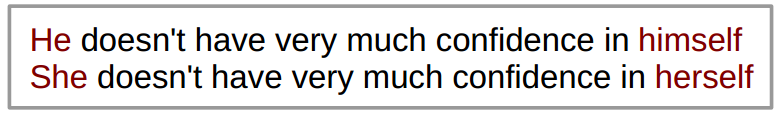
\includegraphics[width=0.7\textwidth]{fig14.png}
\caption{语言中的远距离依存问题示例}
\label{fig:14}
\end{figure}

在讨论循环神经网络之前,先考虑一下前文讲述的语言模型的缺点,当对语言中的所有现象进行建模时,一个基于有限个上文的模型往往捉襟见肘。

在图\ref{fig:14}中,给出了一个远距离句法依存的例子。
在这个例子中,句首的“he”或“her”对句尾的“himself”或“herself”有很强的限定性。
类似的,句子中的动词也会随着句子主语的变化而变化。
不管两个词之间隔了多少个词,这种依存关系是一直存在的,使用一个只考虑有限上文$e_{i-n+1}^{i-1}$的模型,如前文中讨论的那些模型,是无法捕获这种远距离依存关系的。
这种依存关系在英语中恨常见,在俄语等其他语言中更是如此,因为俄语中的词有多种变体形式,而这些变体形式必须和句子中其他成分(词)的性、数、格相对应。

另一个能说明远距离依存关系存在的情况,是\textbf{指代关系\footnote{Selectional Preferences}}\cite{resnik1997selectional}。
简单来说,指代关系指的就是与“什么对什么做了什么”这类问题相关的常识。
举个例子来说,“I ate salad with a fork”中可以很容易的理解“a fork”是一个工具,而“I ate salad with my friend”也是讲得通的,“my friend”可以理解为同伴。
然而,“I ate salad with a backpack”就不怎么讲得通了,因为“backpack”既不是吃饭用的工具,也不是一个同伴。
这种违反指代规则的情况会导致无意义的句子(病句),因为主语、动词、宾语可以相隔很远,所以这种指代相关规则可以跨越很长的范围而起作用。

最后,也有一些句子或文档的\textbf{主题}或\textbf{领域}相关的依存关系。
例如,如果一个文档讨论的是技术主题的内容,突然出现一些体育方面的内容,就会显得很奇怪,即出现了违反主题一致性规则的情况。
再比如,如果一个学术论文突然使用一些不正式的口语化的语言,也会显得极不自然,这就是缺乏领域一致性的情况。

这些例子,当然还可以举出很多其他的例子,都说明了在制作可用的应用软件时,我们之所以需要对语言中远距离依存关系进行建模的原因。

\subsection{循环神经网络}
\textbf{循环神经网络}(RNN;\cite{elman1990finding})是一类神经网络的统称,他们使得对远距离依存关系的建模成为了可能。
模型思路很简单,通过引入一条循环边,在计算当前时刻的隐层状态$\textbf{h}$时将前一时刻的隐层状态$\textbf{h}_{t-1}$也考虑进来,用公式化的语言描述就是:
\begin{equation}\label{eq:44}
 \textbf{h}_t = \left\{ \begin{array}{ll}
  tanh(W_{xh}\textbf{x}_t + W_{hh}\textbf{h}_{t-1}+\textbf{b}_h) & t \geq 0 \\
  \textbf{0} & \textrm{otherwise}
  \end{array} \right.
\end{equation}
我们可以看到,在$t \geq 1$时刻,跟标准的神经网络模型中隐层向量的计算过程的唯一不同之处在于,通过引入$W_{hh}\textbf{h}_{t-1}$项来将$t-1$时刻的隐层状态和$t$时刻的隐层状态连接了起来。
因此,这个函数变成了一个递归函数,即计算过程依赖于前一时刻的隐层状态$\textbf{h}_{t-1}$。
在图\ref{fig:15}(a)中,我们可以看到循环神经网络在当前时刻的计算图拓扑结构。

\begin{figure}[H]
\centering
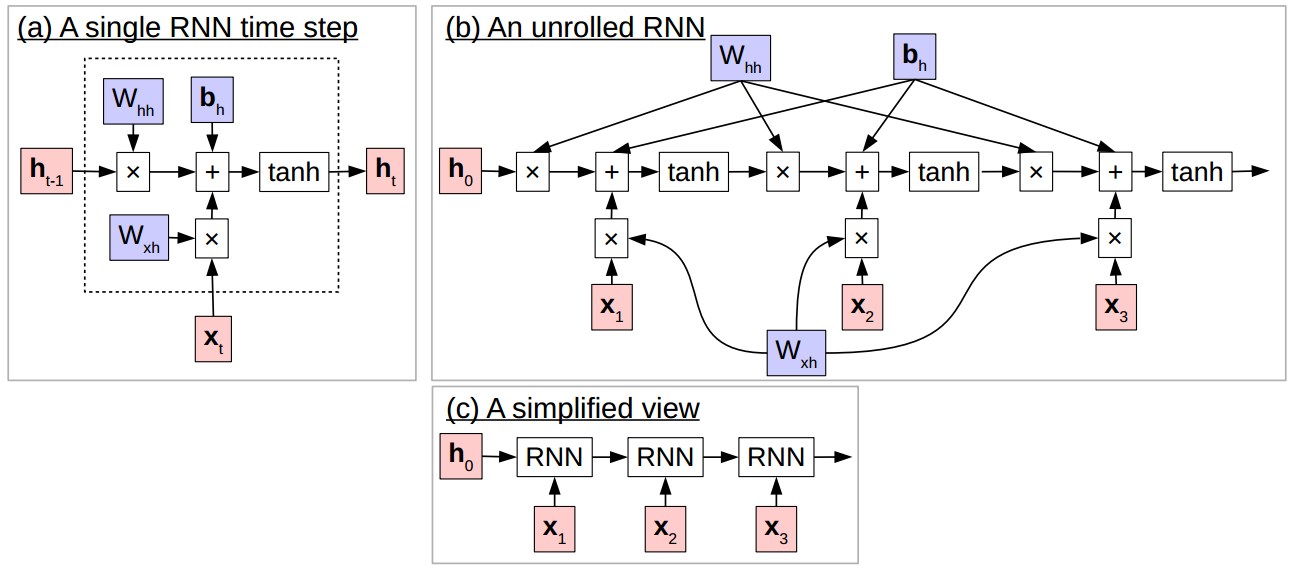
\includegraphics[width=0.9\textwidth]{fig15.png}
\caption{神经网络模型的计算图示例图。(a)给出了单步计算过程。(b)是网络展开后的样子。(c)网络展开后的简化表述形式}
\label{fig:15}
\end{figure}

在对RNN做这样的可视化展现时,通常需要在时间序列上将神经网络进行“循环展开”,就像图\ref{fig:15}(b)中所示的那样,这样能让我们更清晰的看出在多个时刻信息传递的过程。
通过对网络的循环展开,我们可以看到,我们将循环网络的计算过程又规约为了已知的计算图上的计算过程,就像在计算前馈神经网络时所作的那样,在这个展开的计算图拓扑结构上,我们可以进行前向计算和错误的后向传递,进而可以学习模型的参数。
不难看出,循环神经网络必须从一个初始的隐层状态$\textbf{h}_0$开始计算。
这个初始状态一般会被设为一个全零向量,或者被作为参数$\textbf{h}_{init}$通过学习得到,亦或者通过其他信息来对其进行初始化(更多相关讨论见第7节)。

最终,为了简便起见,我们通常把循环神经网络的一个完整计算过程简称为“RNN”计算模块,如图\ref{fig:15}(c)所示。
在这个例子中,对应于RNN函数的方框都是灰色的,意思是他们内部包含了参数$W_{xh}$,$W_{hh}$和$b_h$。
我们会在后面的内容中沿用这种约定俗称的简写形式来表示带参数的函数模块。

由于有了能让信息在不同时刻之间传递的能力,RNN模型使得对远距离依存关系的建模成为了可能。
例如,如果$\textbf{h}_{t-1}$中的某些节点表示了“这个句子的主语是个男性”这样一条信息,可以将这个信息传递到$\textbf{h}_t$,进而传递给$\textbf{h}_{t+1}$,从而能一直传递到这个句子结束为止。
这种在很长的时间序列上传递信息的能力,就是循环神经网络的过人之处,使得这个模型能够解决6.1节中讲述的远距离依存关系的建模问题。

现在,我们已经了解了RNN相关的基础知识,将其应用到语言模型建模过程就变得比较直观了\cite{mikolov2010recurrent}。
我们只需在公式\ref{eq:42}所示的前馈神经网络语言模型中加入一条循环边而得到如下的公式:
\begin{equation}\label{eq:45}
 \begin{array}{l}
 \textbf{m}_t = M_{\cdot,e_{t-1}} \\
 \textbf{h}_t = \left\{ \begin{array}{ll}
  tanh(W_{xh}\textbf{x}_t + W_{hh}\textbf{h}_{t-1}+\textbf{b}_h) & t \geq 0 \\
  \textbf{0} & \textrm{otherwise}
  \end{array} \right. \\
 \textbf{p}_t = softmax(W_{hs}\textbf{h}_t + b_s).
 \end{array}
\end{equation}
在这里值得一提的是,与前馈神经网络语言模型不同,我们在这里只输入前一个词,而不是前驱的两个词。
这是因为,我们期望词条$e_{t-2}$和所有其前面的词的信息已经包含在$\textbf{h}_{t-1}$里了,这样也就不需要直接输入这些前驱词的信息了。

为了表述方便,通常会用$RNN(\cdot)$函数来简化$\textbf{h}_t$的计算公式,如图\ref{fig:15}(c)中RNN的简化画法相对应地,我们可以将上述公式简化为:
\begin{eqnarray}
 \textbf{m}_t & = & M_{\cdot,e_{t-1}} \nonumber \\
 \textbf{h}_t & = & RNN(\textbf{m}_t, \textbf{h}_{t-1}) \nonumber \\
 \textbf{p}_t & = & softmax(W_{hs}\textbf{h}_t + b_s). \label{eq:46}
\end{eqnarray}

\subsection{梯度消失和长短记忆模型}
然而,虽然前一节中介绍的RNN模型在概念上是很简单的,但是它也有自身的问题:一个是\textbf{梯度消失}问题,另一个姊妹问题是\textbf{梯度爆炸}问题。

在图\ref{fig:16}中,给出了梯度消失问题的一个概念化示例。在这个例子中,我们有一个循环神经网络模型,比如是一个用来对文档进行分类的模型,亦或是在给定一段序列文本后进行某种预测行为的模型,会在经过几步RNN操作后做出一个预测行为。
完成这个预测后,就可以计算出损失函数值,并期望这个损失值能够在后向传播过程中传播到神经网络的每个时间节点处。
然而,在每一个时间节点,当我们执行后向传播操作时,梯度值会越来越小,当传播到句子的开始部分时,我们的梯度值会变得极小,以至于对参数更新而言,这个极小的梯度几乎起不到有效的更新作用。
造成这个问题的主要原因,是因为,除非$\frac{d\textbf{h}_{t}}{d\textbf{h}_{t-1}}$的值等于1,否则它就会趋向于让梯度值$\frac{d\mathcal{L}}{d\textbf{h}_t}$变得极小或极度放大,尤其是这种减少或放大行为多次进行后,会对损失函数的梯度造成指数级影响。

\begin{figure}[H]
\centering
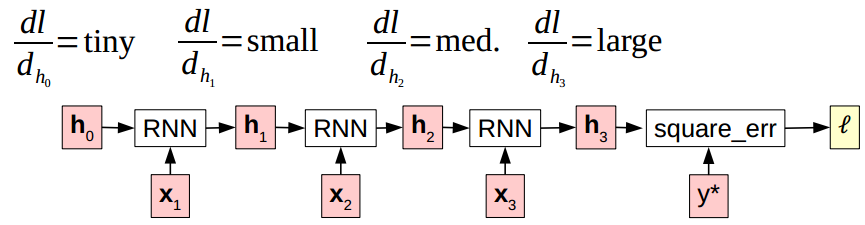
\includegraphics[width=0.7\textwidth]{fig16.png}
\caption{梯度消失问题的一个具体例子}
\label{fig:16}
\end{figure}

一种解决这个问题的方法,比如说解决梯度消失问题的方法,是通过针对性的设计一个神经网络架构来保证循环函数的梯度值为1。
一种被称为\textbf{长短距离记忆}模型(LSTM;\cite{hochreiter1997long})的神经网络架构,就是为这个目的而设计的一个神经网络架构,在多种序列处理问题建模过程中,该模型获得了相当大的成功和极大的关注度。
LSTM模型背后最基本的思想,就是在大多数神经网络常用的标准隐层状态$\textbf{h}$的基础上,它还加入了一个\textbf{记忆单元层}$\textbf{c}$,而它的梯度$\frac{d\textbf{c}_t}{d\textbf{c}_{t-1}}$等于1。
正因为这个梯度值为1,存储在记忆单元的信息不会遭遇梯度消失问题,因此,相比于标准的循环神经网络,LSTM模型能够更有效的捕获远距离依存关系。

\begin{figure}[H]
\centering
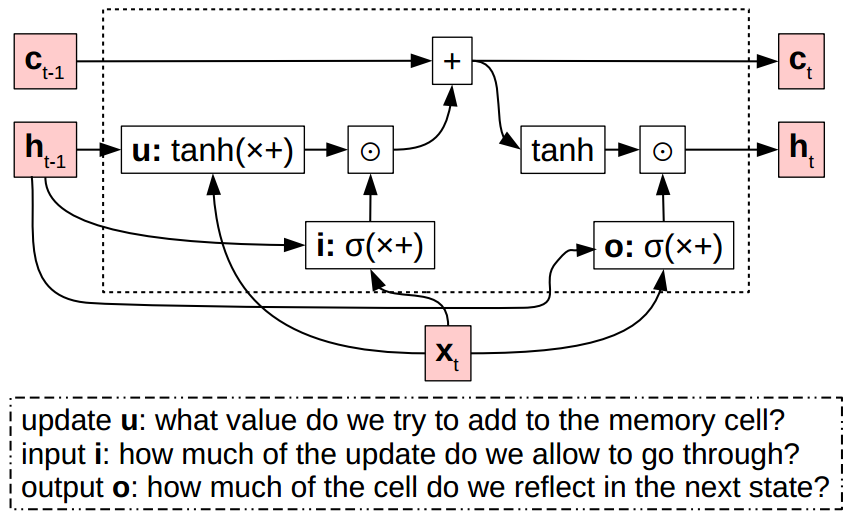
\includegraphics[width=0.7\textwidth]{fig17.png}
\caption{LSTM模型的单步计算过程。隐层\textbf{$h$}和记忆单元\textbf{$c$}之间的信息流通过参数化的输入输出门来控制}
\label{fig:17}
\end{figure}

LSTM模型是如何做到这一点的呢?为了理解其中的奥秘,我们通过图\ref{fig:17}形象而具体地看一下LSTM的架构是怎么样的,下面是其形式化的公式表达:
\[
 \begin{array}{l}
 \textbf{u}_t = tanh(W_{xu}\textbf{x}_t + W_{hu}h_{t-1} + \textbf{b}_u) \\
 \textbf{i}_t = \sigma (W_{xi}\textbf{x}_t + W_{hi}h_{t-1} + \textbf{b}_i) \\
 \textbf{o}_t = \sigma (W_{xo}\textbf{x}_t + W_{ho}h_{t-1} + \textbf{b}_o) \\
 \textbf{c}_t = \textbf{i}_t \odot \textbf{u}_t + \textbf{c}_{t-1} \\
 \textbf{h}_t = \textbf{o}_t \odot tanh(\textbf{c}_t).
 \end{array}
\]
我们一个公式一个公式地看:
公式47是更新函数,基本上和RNN中的更新函数44类似;接收输入向量和隐层状态,执行一次线性变换后经过tanh函数进行非线性化。

公式48和公式49,分别是LSTM模型中的\textbf{输入门}和\textbf{输出门}。“门”所要进行的操作,根据其名字就能看出,就是让信息要么通过这个门,要么被拒之门外而阻断其传播。这两个门都进行一次线性变换然后经过\textbf{sigmoid函数},这个函数也被称为\textbf{逻辑斯蒂函数}:
\[
 \sigma (x) = \frac{1}{1 + exp(-x)}
\]
这个函数将输入值$x$压缩到0至1的范围内,当$x$的值趋向于负无穷时$\sigma(x)$的值会趋向于0,当$x$的值趋向于正无穷时$\sigma(x)$的值会趋向于1。Sigmoid函数的输出,会用来和另一个函数的输出结果进行分量型乘法操作:
\[
 \begin{array}{l}
 \textbf{z} = \textbf{x} \odot \textbf{y} \\
 z_i = x_i * y_i
 \end{array}
\]
“门”效应的结果:如果向量的某个维度的sigmoid结果接近1,这个点上对输入没有什么影响(即这个门处于“开启”状态),如果其sigmoid值接近0,则这个输入会被阻截,导致乘积结果为0(即这个门处于“关闭”状态)。

公式50是LSTM模型中最重要的公式,因为它是“让梯度$\frac{d\textbf{c}_t}{d\textbf{c}_{t-1}}$必须等于1”这个直观目的的实现细节,也正是我们解决梯度消失问题的关键步骤。这个公式让$\textbf{c}_t$的值等于输入门$\textbf{i}_t$和更新门$\textbf{u}_t$的外积加上前一个时间节点的$\textbf{c}_{t-1}$。因为我们是直接将$\textbf{c}_{t-1}$作为了计算$\textbf{c}_t$时的一个加和项,如果我们只看公式50中的这个加和部分,不难看出这里的梯度$\frac{\frac{d\textbf{c}_t}{d\textbf{c}_{t-1}}}{}$确实为1。

最后,公式51用来计算LSTM的下一个隐层状态。计算过程如下,先将记忆单元的值通过tanh函数变换到-1到1范围内,然后将结果和输出门的结果$\textbf{o}_t$进行外积。这个隐层状态值会在后续的计算过程中用到,比如用于计算语言模型的概率分布:
\[
 \textbf{p}_t = softmax(W_{hs}\textbf{h}_t + b_s)
\]

\subsection{RNN的其他变种}
由于在多个应用中都证明了循环神经网络的重要性,于是有了这种神经网络的多种变体存在。对标准的LSTM模型的一个常见改进模型是引入一个\textbf{忘却门}\cite{gers2000learning},实际上,这个改进版的模型已经常见到,当人们说“LSTM”模型时都指的是这个改进版本。带忘却门的LSTM的相关公式如下:
\[
 \begin{array}{l}
 \textbf{u}_t = tanh(W_{xu}\textbf{x}_t + W_{hu}h_{t-1} + \textbf{b}_u) \\
 \textbf{i}_t = \sigma (W_{xi}\textbf{x}_t + W_{hi}h_{t-1} + \textbf{b}_i) \\
 \textbf{f}_t = \sigma (W_{xf}\textbf{x}_t + W_{hf}h_{t-1} + \textbf{b}_f) \\
 \textbf{o}_t = \sigma (W_{xo}\textbf{x}_t + W_{ho}h_{t-1} + \textbf{b}_o) \\
 \textbf{c}_t = \textbf{i}_t \odot \textbf{u}_t + \textbf{f}_t \odot \textbf{c}_{t-1} \\
 \textbf{h}_t = \textbf{o}_t \odot tanh(\textbf{c}_t).
 \end{array}
\]
跟标准的LSTM模型相比,这里有两处变化。首先来看公式54,我们引入了忘却门。其次,在公式55中,在将前一时刻的$c_{t-1}$传给当前时刻的$c_t$之前用忘却门的结果去与之做个外积。忘却门在一些情况下非常有用,当需要时忘却门能让记忆单元轻易地清空记忆内容,比如,我们不妨假设这个模型记住了一个特定的词条和另一个词条有很强的相关性,比如上个例子中的“he”和“himself”,或者“she”和“herself”。在这个例子中,我们期望模型能够在预测“himself”之前都一直记忆“he”的信息,而预测结束后就忘却这个信息,就好像那两个词再也不相关了一样。忘却门就有这种优势,它能让这种精细的信息流控制成为可能,当然它也带着一个隐患随行,如果$\textbf{f}_t$在每个时刻都被置为0,这个模型会忘却所有信息进而失去捕获远距离依存关系的能力。因此,在开始训练神经网络模型之前,通常都会讲忘却门的偏执参数$\textbf{b}_f$初始化为一个较大的值(比如1),这样能保证神经网络在开始训练时是不会用到忘却门的,随着训练过程的进行,慢慢地开始忘却一些内容。

虽然LSTM模型为梯度消失问题提供了一个有效的解决途径,但这个模型还是太复杂了(很多读者肯定已经感受到了)。另一个简单的RNN变体是基本已被证明有效的\textbf{gated recurrent unit}(GRU;\cite{chung2014empirical}),其形式化公式如下:
\[
 \begin{array}{l}
 \textbf{r}_t = \sigma (W_{xr}\textbf{x}_t + W_{hr}h_{t-1} + \textbf{b}_r) \\
 \textbf{z}_t = \sigma (W_{xz}\textbf{x}_t + W_{hz}h_{t-1} + \textbf{b}_z) \\
 \tilde{\textbf{h}}_t = tanh(W_{xh}\textbf{x}_t + W_{hh}(\textbf{r}_t \odot \textbf{h}_{t-1}) + \textbf{b}_h) \\
 \textbf{h}_t = (1 - \textbf{z}_t)\textbf{h}_{t-1} + \textbf{z}_t \tilde{\textbf{h}}_t.
 \end{array}
\]
GRU模型最独特的一点就是公式59,即对已更新的隐层状态$\tilde{\textbf{h}}_t$和前一时刻的状态$\tilde{\textbf{h}}_{t-1}$进行插值。
这个插值过程受到\textbf{更新门$z_t$}的控制,当更新门的值趋近1时,GRU会使用最新的隐层状态,而当更新门的值趋近0时,它就会使用前一时刻的隐层状态。隐层状态候选的计算过程如公式58所示,和标准的RNN更新过程类似,但它包含了一步操作,即用公式56计算出的\textbf{重置门$r_t$}来对前一时刻的隐层状态输入进行外积。跟LSTM相比,GRU包含的参数稍微少一些,并且没有单独的“记忆单元”的概念。因此GRU模型常常被用来减少内存和计算方面的开销。

\begin{figure}[H]
\centering
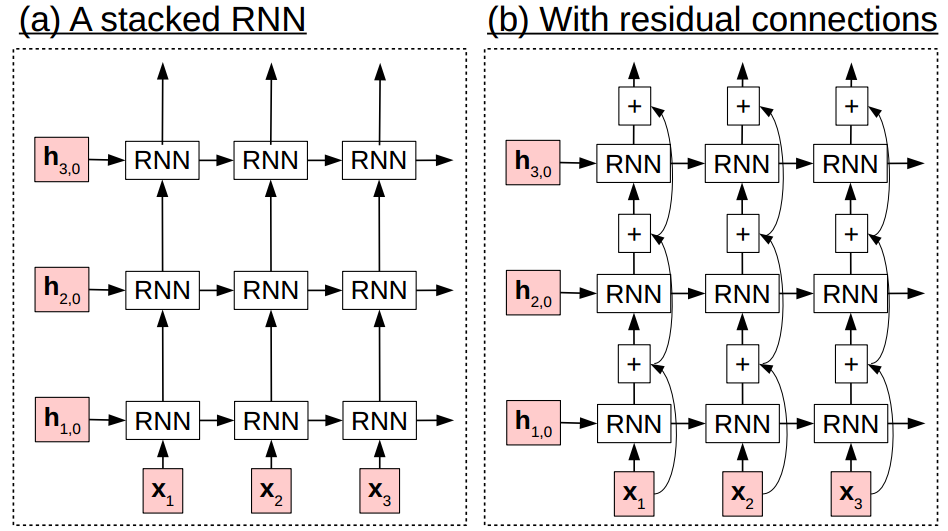
\includegraphics[width=0.8\textwidth]{fig18.png}
\caption{示例图(a)堆叠RNN(b)有残差连接的堆叠RNN}
\label{fig:18}
\end{figure}

我们可以对RNN模型、LSTM模型、GRU模型或者任何神经网络层做一个简单但是非常有效的改进:将多个层一个个堆叠起来(\textbf{多层RNN模型}如图\ref{fig:18}(a))。例如,在一个3层RNN模型中,在$t$时刻的计算过程会如下进行:
\[
 \begin{array}{l}
 \textbf{h}_{1,t} = RNN_1 (\textbf{x}_t,\textbf{h}_{1,t-1}) \\
 \textbf{h}_{2,t} = RNN_2 (\textbf{h}_{1,t},\textbf{h}_{2,t-1}) \\
 \textbf{h}_{3,t} = RNN_3 (\textbf{h}_{2,t},\textbf{h}_{3,t-1}),
 \end{array}
\]
这里$\textbf{h}_{n,t}$是第$n$层在第$t$时刻的隐层状态,而$RNN(\cdot)$是对公式44中的RNN函数计算过程的简称。
类似的,我们可以将这个函数替换为$LSTM(\cdot)$,$GRU(\cdot)$,或者任何其他的循环网络函数。
之所以将多层神经网络堆叠起来会很有用,是因为在第5节介绍的标准神经网络中的非线性变换被证实是非常有用的:它们可以从当前的词或句子中逐层抽取出更加抽象的特征信息。例如,据文献\cite{shi2016does}研究发现,在一个双层的LSTM中,第一层会倾向于学习诸如词性的词的细粒度特征,而第二层会学到诸如句子的音色时态等更抽象的特征。

虽然堆叠的RNN模型具有很多潜在的好处,但也有一些不足之处,比如会遭遇纵向的梯度消失问题,就跟标准的RNN模型在横向上遇到的梯度消失问题一样。那也就是说,梯度会从接近输出层的$RNN_3$反向传播到接近输入层的$RNN_1$,在这个传播过程中梯度可能会消失,导致整个网络的前几层训练不到位。和LSTM解决梯度消失问题的方法类似,解决这个问题也有一个简单的策略,叫\textbf{残差网络(residual networks)}(如图\ref{fig:18}(b))\cite{he2016deep}。这些网络架构背后的思想其实比较简单,就是将前一层的输出加到当前层的输出上,就像下面的公式所述:
\[
 \begin{array}{l}
 \textbf{h}_{1,t} = RNN_1 (\textbf{x}_t,\textbf{h}_{1,t-1}) + \textbf{x}_t \\
 \textbf{h}_{2,t} = RNN_2 (\textbf{h}_{1,t},\textbf{h}_{2,t-1}) + \textbf{h}_{1,t} \\
 \textbf{h}_{3,t} = RNN_3 (\textbf{h}_{2,t},\textbf{h}_{3,t-1}) + \textbf{h}_{2,t}.
 \end{array}
\]
这样一来,就像LSTM一样,就不存在梯度传播过程中因为经过$RNN(\cdot)$函数而消失的问题,即使是很深的网络架构也会有效的学习到每层的参数。

\subsection{实时,整块,小块训练}
善于观察的读者可能已经注意到了,前一节中循序渐进的介绍了一个比一个复杂的模型,我们从一个简单的线性模型开始,加入了一个隐层,又加入了循环性,加入了LSTM,然后加入了多层的LSTM。虽然这些更有表达性的模型有能力达到更高的精度,但这也是有代价的:大幅增长的参数空间(导致极有可能过拟合)和更加复杂的运算过程(导致需要更多的计算消耗)。本节将介绍一种能提升训练这些复杂模型的稳定性以及计算效率的有效方法,\textbf{minibatching}。

到目前为止,我们已经用了4.2节中介绍过的随机梯度下降学参算法,其更新过程可以描述为下面的迭代过程。每次根据一个样本来进行参数学习更新的这类学习方法,我们称之为\textbf{online learning}。

\begin{figure}[H]
\centering
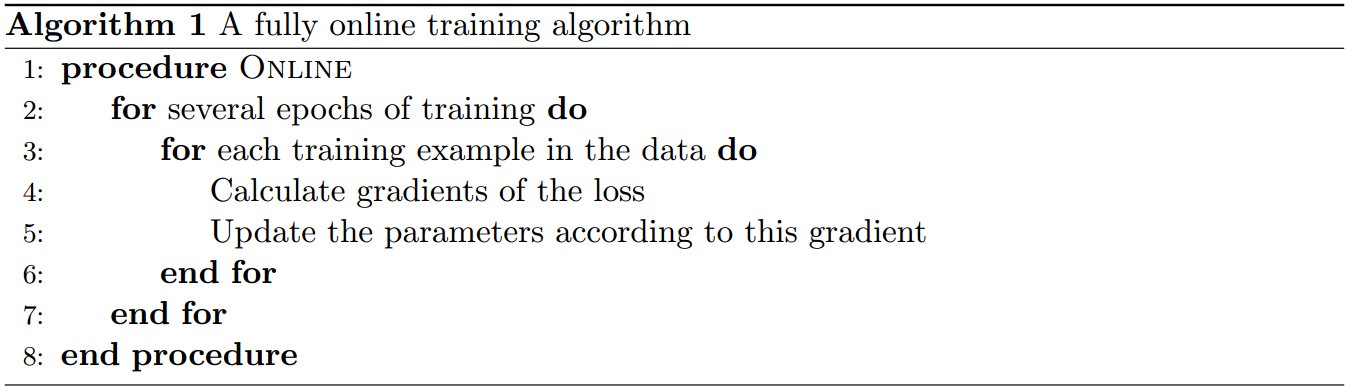
\includegraphics[width=1\textwidth]{alg1.png}
\end{figure}

相反地,我们也可以想到\textbf{batch learning}算法,这种学习方法会将这个训练数据作为一个单元,在这个整体单元上计算梯度值,每次遍历完整个训练数据后才进行参数更新。

这两种更新策略需要进行折中考虑。
\begin{itemize}
\item 因为不需要遍历完整的数据就可以进行参数更新,所以在线学习算法通常能更快地找到相对更好的解。
\item 然而,由于不会受最近看到的训练样本的过度影响,在训练快要结束的阶段,批量学习算法会更稳定。
\item 批量学习算法也更容易陷入局部最优;在线学习中的随机机制,可以让其能够跳出局部最优点从而找到更好的全局解。
\end{itemize}

\begin{figure}[H]
\centering
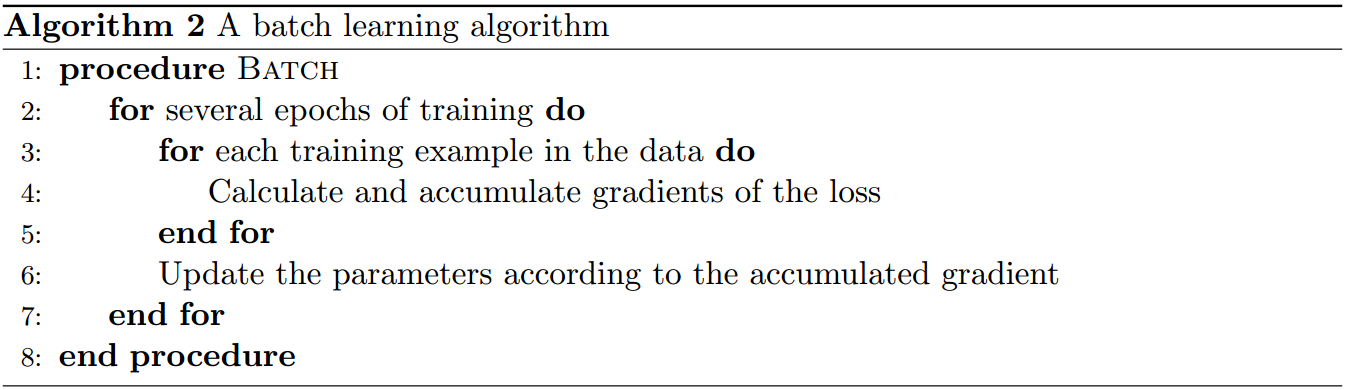
\includegraphics[width=1\textwidth]{alg2.png}
\end{figure}

\begin{figure}[H]
\centering
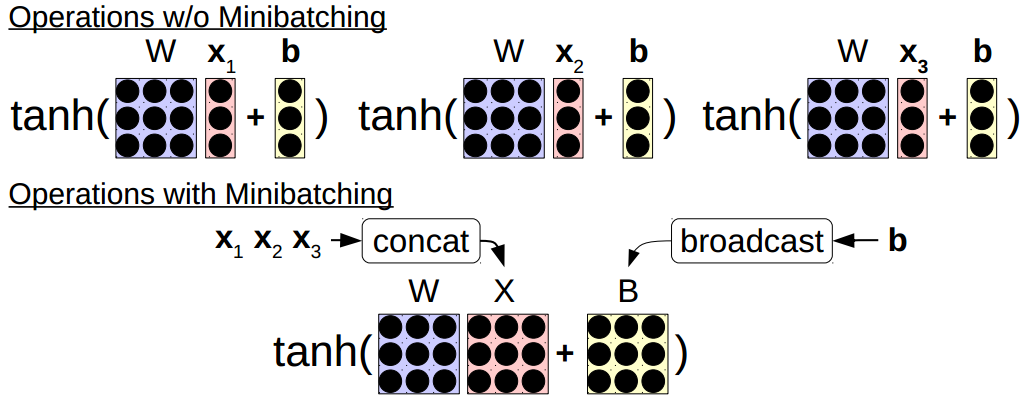
\includegraphics[width=0.8\textwidth]{fig19.png}
\caption{在小块训练过程中合并多个相同操作的一个示意图}
\label{fig:19}
\end{figure}

小块训练方法是这两种策略的一个很好的折中。基本上,小块训练和在线学习过程相似,只不过在每次学习参数时不再是只考虑一个样本,而是考虑$n$个样本来计算这些样本整体的梯度。在$n=1$这个特殊情况下,这种学习方法就跟在线学习是一样的了,而当$n$等于整个训练数据的大小时,这种学习方法又等同于批量学习方法。在训练语言模型时,每次参数更新前需要学习$n=1$到$n=128$个句子来作为数据块。当我们增加训练样本数时,每次参数更新过程会更有信息量且更稳定,但每轮更新参数所消耗的时间也会增加,所以,通常我们会从这两个方面的平衡的角度出发去选择$n$的大小。

小块训练方法的另一个主要益处是:通过使用一些小技巧,可以让同时处理$n$个训练样本所消耗的时间比单独处理$n$个样本所消耗的时间要少的多。具体地,当我们同时处理多个训练样本且将计算过程中相同的操作分组同时处理时,我们可以得到更大的计算效率上的增益,这是因为有这样一个事实的存在,现在的硬件设备(特别是GPU,当然也包括CPU)拥有非常有效率的向量处理指令,可以利用适当结构化的输入数据来提升计算效率。如图\ref{fig:19}所示,在神经网络中的这种操作重组的例子包括:把多个训练样本上的矩阵和向量相乘的过程组合为矩阵和矩阵相乘的过程,或者,在多个向量上同时进行诸如tanh等原子操作,而不是一个向量一个向量地单独计算。幸运的是,在我们所使用的DyNet包中,做到这一点相对比较容易,因为很多这种机械的原子操作都会被自动的归并处理。我们将在下文中给出一个示例,来说明当我们实现一个RNN语言模型时如何来做这些改进优化。

\begin{figure}[H]
\centering
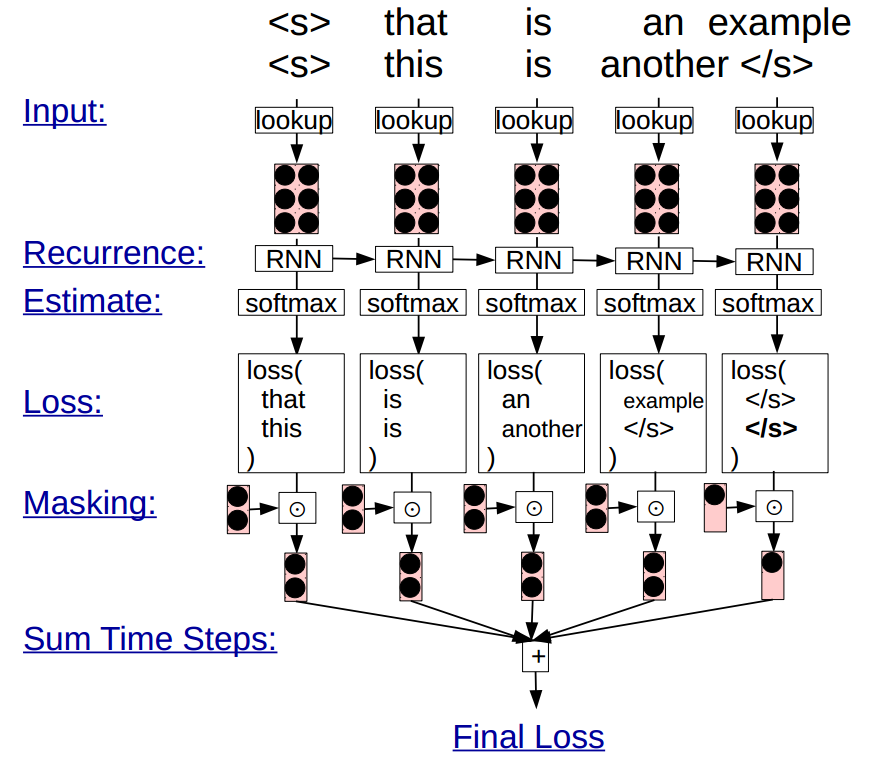
\includegraphics[width=0.8\textwidth]{fig20.png}
\caption{RNN语言模型中的小块训练过程样例}
\label{fig:20}
\end{figure}

小块RNN语言模型(图\ref{fig:20})的基本思想是这样的,我们一次性处理多个句子,而不是每次处理一个句子。因此,我们需要同时查找多个词的词向量,而不是一个词一个词的查其向量表示。然后我们向正常情况下那样将这些成块儿的词向量输入到RNN和softmax函数中,得到两个独立的概率分布,分别表示第一句和第二句中的词的概率分布。然后我们计算每个词的损失函数值。我们将这些损失值加起来作为整个句子的损失值。

然而,还有一个具体问题,那就是,如图中所示的那样,我们所造出来的小块数据里很可能存在不同长度的句子。在这种情况下,为了确保能够正常处理不同长度的句子,通常需要进行\textbf{句子补全}和\textbf{masking}操作。句子补全操作很简单,就是在小块中长度较短的句子后面加上一个或多个“句末符”,从而使其长度和这块数据中最长的句子相等,这样就保证了同一块数据中所有句子都是等长的了。Masking是这样进行的,对前面所述的人为添加的“句末符”,在计算损失函数值时要乘以0,这样就确保了短句中的多个句末符不会被重复计算损失值。

通过这样两个操作,我们就可以同时处理不等长的多个句子了,但任然有一个问题:如果我们的小块数据中的句长差异很大,那我们就需要人为添加很多的句末符来填充位置,而过多的句末符填充,就会浪费过多的计算资源。为了解决这个问题,通常会对训练语料中的句子按句子长度进行排序,然后在制作小块,来确保每个小块中的句子都差不多是等长的。

\subsection{扩展阅读}
因为RNN模型在包括自然语言和其他数据的多个处理应用中都很受欢迎,因此对其扩展的兴趣一直比较大。下面列几个人们正在着手研究的课题:
\begin{enumerate}
\item[] \textbf{循环神经网络能学到什么?}RNN是用来处理语言的十分强大的工具,因此很多研究人员都对其内部到底在发生什么很感兴趣。文献\cite{karpathy2015visualizing}展示了对LSTM网络内部状态的几种可视化方法,发现有些节点会负责跟踪句子的长度,或者是是否开启了括号,或者其他显著的句子特征。文献\cite{li2015visualizing}给出了几种方法,通过在基于RNN的模型在其神经网络上向后传递的信息,来分析和可视化对模型最终判定起决定性贡献的输入部分。
\item[] \textbf{其他的RNN架构:}还有很多其他的循环神经网络架构。文献\cite{greff2016lstm}进行了一项很有意思的研究,他们通过对LSTM的不同部分进行去除的研究,来查找针对具体任务而言最好的神经网络架构。文献\cite{zoph2016neural}在这个基础上更进一步,具体地训练一个模型,来查找这种最优的神经网络架构。
\end{enumerate}

%\subsection{练习}


\section{神经编码-解码模型}
从第3节到第6节,我们把关注点放在了用于计算一个序列$E$的概率分布$P(E)$的语言模型问题上。在本节中,我们回到统计机器翻译问题上来,即在给定输入$F$的情况下计算输出$E$的概率分布$P(E | F)$的建模问题。

\subsection{编码-解码模型}
我们将介绍的第一个模型是\textbf{编码-解码}模型\cite{chrisman1991learning,forcada1997recursive,kalchbrenner2013recurrent,sutskever2014sequence}。这个模型背后的基本思想相对来说比较简单:我们有一个RNN语言模型,但在开始计算$E$的概率分布之前,我们先用另一个RNN模型在源语言句子$F$上计算出这个模型的每一个内部隐层状态。“编码-解码”这个名字是从这样一个概念而得来的,第一个神经网络将源语言句子$F$的信息“编码”成一个实数值向量(隐层状态向量),然后第二个神经网络把这个信息“解码”为目标语言句子$E$。

\begin{figure}[H]
\centering
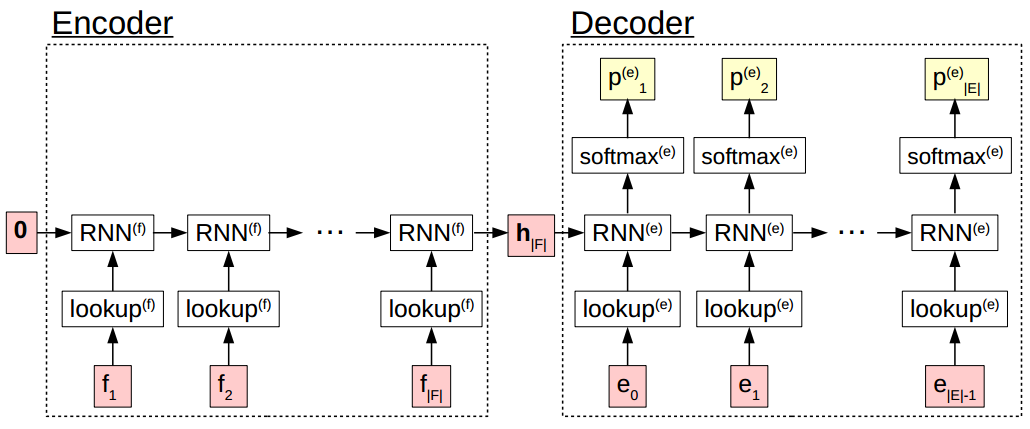
\includegraphics[width=0.8\textwidth]{fig21.png}
\caption{编码-解码模型的一个计算图示例}
\label{fig:21}
\end{figure}

如果我们用$RNN^{(f)}(\cdot)$来表示这个编码器,用$RNN^{(e)}(\cdot)$来表示这个解码器,然后,我们还有个softmax函数来接收$RNN^{(e)}$在时刻$t$的隐层状态作为输入来将其转换成概率分布,那么,我们的模型可以描述为如下几个公式(如图\ref{fig:21}所示):
\[
 \begin{array}{l}
   \textbf{m}_t^{(f)} = M_{\cdot,f_t}^{(f)} \\
   \textbf{h}_t^{(f)} = \left\{ \begin{array}{ll}
      RNN^{(f)}(\textbf{m}_t^{(f)},\textbf{h}_{t-1}^{(f)}) & t \geq 1 \\
      \textbf{0} & \textrm{otherwise}
      \end{array} \right. \\
   \textbf{m}_t^{(e)} = M_{\cdot,e_{t-1}}^{(e)} \\
   \textbf{h}_t^{(e)} = \left\{ \begin{array}{ll}
      RNN^{(e)}(\textbf{m}_t^{(e)},\textbf{h}_{t-1}^{(e)}) & t \geq 1 \\
      \textbf{h}_{|F|}^{(f)} & \textrm{otherwise}
      \end{array} \right. \\
   \textbf{p}_t^{(e)} = softmax(W_{hs}\textbf{h}_t^{(e)} + b_s)
 \end{array}
\]
在前两行,我们查到词向量$\textbf{m}_t^{(f)}$然后计算编码器在源语言句子$F$上第$t$时刻的隐层状态$\textbf{h}_t^{(f)}$。
我们从一个零向量$\textbf{h}_0^{(f)}=\textbf{0}$作为初始状态来开始计算,而当计算到$\textbf{h}_{|F|}^{(f)}$时,编码器已经把源语言句子中的所有词都遍历完了。因此,这个隐层状态在理论上是对源语言句子中的信息的编码结果了。

在解码阶段,我们在每个时刻预测词条$e_t$的概率分布。首先,类似地,我们先查找词向量$\textbf{m}_t^{(e)}$,但是我们这次试用前一个词$e_{t-1}$,因为我们必须把$e_t$的概率分布建立在前一个词$e_{t-1}$的条件上,而不是以自己作为条件。然后,我们用解码器来计算其隐层状态$\textbf{h}_t^{(e)}$。这一计算过程和编码阶段的计算过程很类似,唯一不同在于,为了让解码器在给定$F$的条件下进行计算,我们把解码器的初始状态$\textbf{h}_0^{(e)}$设为编码器的最终状态$\textbf{h}_{|F|}^{(f)}$。最后,我们用softmax函数在隐层状态$\textbf{h}_t^{(e)}$上计算概率分布$\textbf{p}_t^{(e)}$。

虽然这个模型相当简单(只有5行公式而已),但给了我们提供了对$P(E|F)$建模的一个直观且强大的方法。
事实上,\cite{sutskever2014sequence}指出,这样一个简单的模型也能进行翻译操作,其翻译效果甚至和那些针对机器翻译任务而经过特别重度优化过的系统一样好。

\subsection{生成结果}
到目前为止,我们只提到了如何创建一个概率模型$P(E|F)$,但没有讲述如何用这个概率模型来生成翻译结果,而这也是我们下一小节将讨论的内容。简单来说,我们可以使用如下几种方法来生成翻译结果:
\begin{enumerate}
\item[] \textbf{随机采样:}从概率分布$P(E|F)$上随机选择一个翻译输出$E$。通常把这个工程表示为$\hat{E} \sim P(E|F)$。
\item[] \textbf{1-best搜索:}搜索一个$E$使得$P(E|F)$最大化,表述为$\hat{E} = \arg\max \limits_{E} P(E|F)$。
\item[] \textbf{n-best搜索:}搜索概率值$P(E|F)$最高的$n$个翻译候选结果。
\end{enumerate}
选择哪种方法来生成翻译结果,我们需要依据具体的应用需求而定,因此我们将在介绍具体算法的同时会顺带着介绍一些使用样例。

\subsubsection{随机采样}
当我们需要对同一个输入得到多个不同的输出时,\textbf{随机采样}是个很有用的方法。一个这种方法很有用的使用情景,是用端到端模型来处理对话系统的情况,因为我们不希望对话系统对用户的同一个输入内容总是回复相同的回答,即不希望系统的回答不那么单调。幸运的是,在上述的编码-解码模型中,从概率分布$P(E|F)$采样生成候选是非常简单的事,有一种叫做\textbf{祖采样}的方法就能帮我们做到这一点。祖采样过程是这样进行的,在每个时间点采样多个样本,逐步扩展上文内容,在第$t$时刻,我们从概率分布$P(e_t | \hat{e}_1^{t-1})$中采样出一个词。在编码-解码模型中,这意味着我们只需要根据前面采样出来的输入来计算概率$\textbf{p}_t$,就引出了如【】所示的简单的生成算法。

值得一提的是,有时候我们想要知道我们采样出来的句子的概率值。例如,对于模型生成的一个句子$\hat{E}$,我们想要知道模型对于它所生成的这句话的置信度。在采样过程中,我们可以通过循序渐进的通过将每一个采样出来的词的概率相乘来计算句子概率$P(\hat{E}|F) = \prod_{t}^{|\hat{E}|}P(\hat{e}_t|F,\hat{E}_1^{t-1})$。然而,我们还记得在3.3节讨论的概率与对数概率的情况吧,直接使用概率值来计算常常会在计算机系统中产生浮点数溢出的问题。因此,在计算整句话的概率时,为了防止这种浮点数溢出问题的出现,通常都会将概率乘积换成对数概率之和的方法来计算。

\begin{figure}[H]
\centering
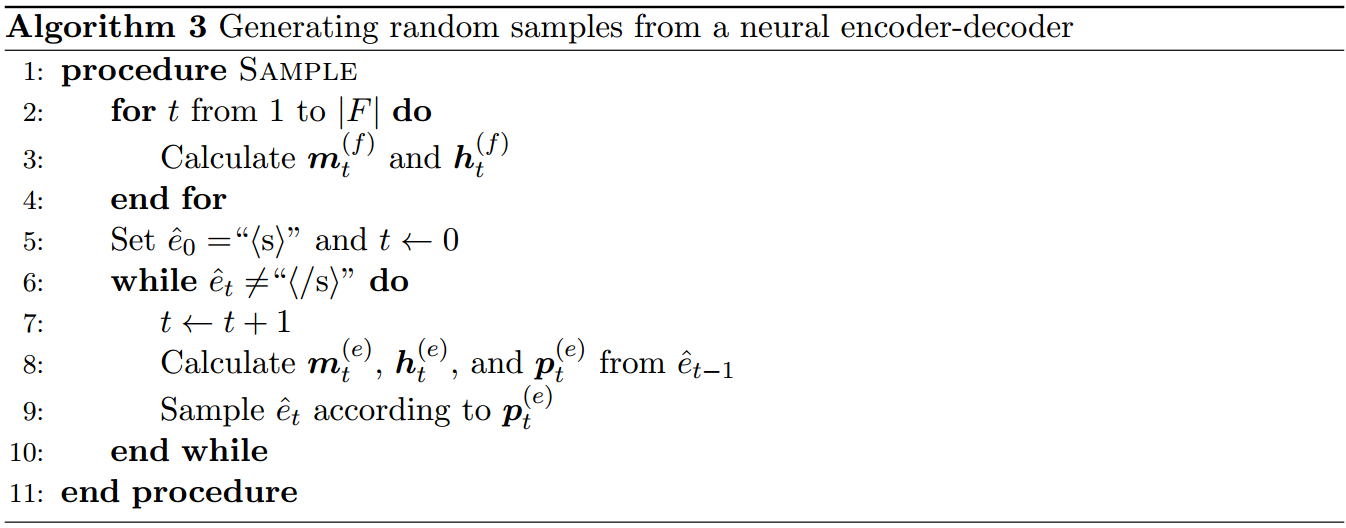
\includegraphics[width=1\textwidth]{alg3.png}
\end{figure}

\subsubsection{贪心1-best搜索}
下面,我们来考虑生成1-best最佳结果的问题。这种生成方式,在机器翻译这种我们只想让模型输出它认为最佳的译文的应用中非常有用。
最简单的做法就是\textbf{贪心搜索},即,在每个时刻计算出概率分布$\textbf{p}_t$,从这个分布中选择概率最大的那个词,然后将这个词作为结果序列中的下一个词。换句话说,这个生成算法和算法3完全一样,区别只是在第9行上,在这里我们选择最大概率词$\hat{e}_t = \arg \max \limits_{i} p_{t,i}^{(e)}$,而不是根据概率分布$\textbf{p}_t^{(e)}$来随机采样出$\hat{e}_t$。

有趣的是,祖采样方法能按照概率分布$P(E|F)$精确的采样出输出结果,贪心搜索却不能保证能搜索到概率最大的译文。
在图\ref{fig:22}中,可以看到一个能说明这是事实的一个样例,这个示例是一个词表为\{a,b,</s> \}的搜索图。作为练习,我鼓励读者去找一下给定概率分布$P(E|F)$时的真实的1-best(或n-best)句子出来,再计算一下贪心搜索得到的结果句子的概率值,来证实一下他们是不同的。

\begin{figure}[H]
\centering
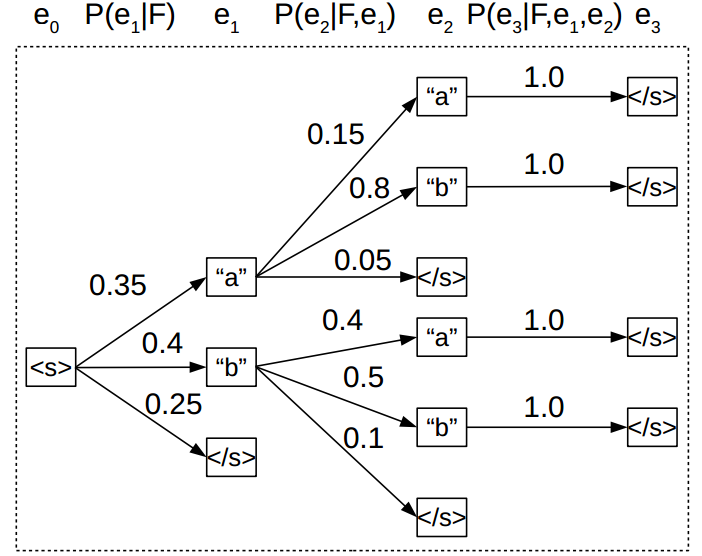
\includegraphics[width=0.7\textwidth]{fig22.png}
\caption{贪心搜索会失败的一个搜索过程图样例}
\label{fig:22}
\end{figure}

\subsubsection{Beam Search}
解决这个问题的一种方法是\textbf{Beam Search}。Beam Search和贪心搜索方法类似,但和贪心搜索在每个时刻只考虑一个最佳翻译假设不同,beam search在每个时刻考虑$b$个最佳翻译假设,这里$b$是beam的“深度”。在图\ref{fig:23}中给出了一个$b=2$时的beam search过程。
在第一个时刻,我们用词表中的这三个词来扩展$e_1$的翻译假设,然后保留得分排在前两个的候选(“b”和“a”)而删除剩下的那一个(“</s>”)。在第二个时刻,我们继续用词表中的词来扩展$e_2$的翻译假设,临时性生成$b * |V|$个假设。这些假设也会被剪枝到剩下$b$个有效假设(“ab”和“bb”)。先展开$b * |V|$个假设并计算其得分,然后剪枝到得分排在前$b$个的候选假设,这个操作过程会一直持续到整个句子生成结束为止。

\begin{figure}[H]
\centering
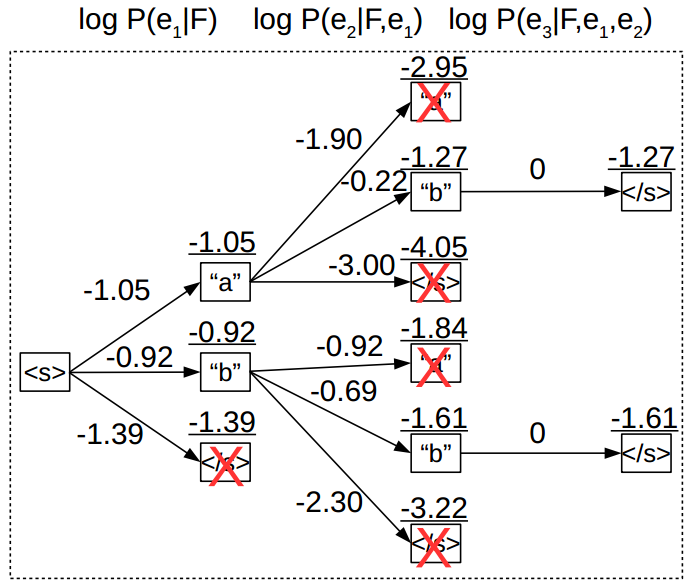
\includegraphics[width=0.7\textwidth]{fig23.png}
\caption{栈大小$b=2$的一个栈搜索样例。}
\label{fig:23}
\end{figure}

在使用神经网络机器翻译模型等模型来生成句子时,需要注意一点,根据概率$P(E|F) = \prod_t^{|E|}P(e_t | F,e_1^{t-1})$来看,模型会倾向于生成短句。这是因为,每次我们给生成结果中加入另一个词时,其概率值都会被乘以一个概率值,从而降低了整个句子的概率值。当我们加大beam大小时,搜索算法会更容易找到这些短句,因此,beam大小较大的beam search算法对这些更短的句子有显著的\textbf{length bias}。

很多方法都在尝试解决这个长度偏执问题。例如,可以根据给定的源语言句子长度来设置一个生成句子长度的先验概率$P(|E| | |F|)$,然后在解码阶段,将这个概率和标准的句子概率$P(E | F)$相乘而得到\cite{eriguchi2016tree}:
\[
 \hat{E} = \arg \max \limits_{E} \log P(|E|||F|) + \log P(E|F).
\]
这个先验概率可以在训练数据中统计得到,文献\cite{eriguchi2016tree}通过在训练语料上统计到的多项分布来作为这个先验概率的估计值:
\[
 P(|E|||F|) = \frac{c(|E|,|F|)}{c(|F|)}.
\]
一个更具启发性但仍广泛被使用的方法,是用目标句子的长度来对其对数概率值进行归一化处理,有效地搜索平均每个词的概率对数最高的译文\cite{cho2014properties}:
\[
 \hat{E} = \arg \max \limits_{E} \log P(E|F)/|E|.
\]

\subsection{序列编码的其他方法}
在7.1小节,我们描述了一个模型,这个模型从左到右一个词一个词地将这个线性序列编码。然而,这可能不是将句子$F$转换成向量$\textbf{h}$的最自然或最有效的方式。在本节内容中,我们将讨论一系列不同的编码方法,这些方法都曾在文献中被证明是有效的。

\subsubsection{倒序和双向编码}
首先,文献\cite{sutskever2014sequence}提出了\textbf{逆向编码器}。在这个方法中,我们让句子$F$通过一个标准的线性编码器,这次是从右到左的顺序来编码,而不是原来那样从左到右进行编码。
\[
 \overleftarrow{h}_t^{(f)} = \left \{ \begin{array}{ll}
  \overleftarrow{RNN}^{(f)}(\textbf{m}_t^{(f)},\textbf{\overleftarrow{h}}_{t+1}^{(f)}) & t \leq |F| \\
  \textbf{0} & \textrm{otherwise.}
 \end{array} \right.
\]

\begin{figure}[H]
\centering
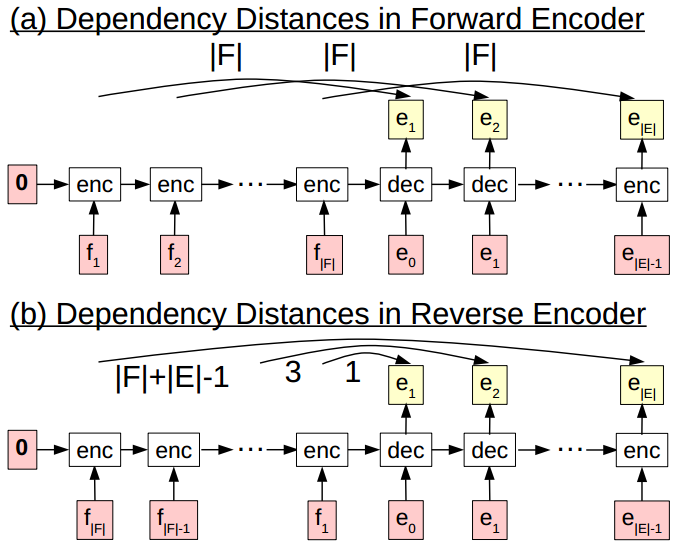
\includegraphics[width=0.7\textwidth]{fig24.png}
\caption{在正向和反向解码器中,相同位置的词之间的距离}
\label{fig:24}
\end{figure}

这个方法背后的思想,对于词序相似的两种语言(比如英语和法语),句子$F$的第一个词很大程度上与句子$E$的第一个词相对应。假设一种极端情况,即两个句子中每个位置的词都一一对应(如,$f_1$对应于$e_1$,$f_2$对应于$e_2$,以此类推),在线性编码和解码过程中,对应的两个词之间的距离是$|F|$,如图\ref{fig:24}(a)所示。还记得6.3节所讲的梯度消失问题吧,这意味着RNN模型需要在作出预测之前,要将所携带的信息传播经过$|F|$个时刻,这是非常困难的事情。在训练开始时,即使是RNN的变种的LSTM模型也会遇到问题,因为它们需要在没有先验偏执的情况下猜测隐层状态中编码的哪一部分信息是可以利用的。

将编码过程的方向逆过来可以解决这个问题,因为这样一来就缩短了句子中部分词之间的依赖距离,尤其是句首的那些词。如图\ref{fig:24}(b)所示,$f_1$和$e_1$之间的依赖距离为1,$f_t$和$e_t$之间的距离为$2t-1$。在训练过程中,模型可以“锁定”到这些短距离依赖,并将其作为引导训练过程的一种方式,之后便有可能循序渐进的学习到句末词之间的更远距离的依赖关系。在\cite{sutskever2014sequence}中,这个方法被证明是编码-解码模型架构的关键所在。

然而,这个将编码过程的方向逆过来的方法,建立在一个很强的假设之上,即,输入的句子和输出的句子中的词序是非常相似的,或者说至少在句首部分的词序是一样的。这个假设对于像英语和法语这样的语言是对的,因为这两种语言都是“主-谓-宾(SVO)”结构的,但对于其他类型的语言来说就未必成立了。有一种对不同类型语言更加鲁棒一些的编码器是\textbf{双向编码器}\cite{bahdanau2014neural}。在这个方法中,我们使用两个不同的编码器:一个负责对输入的句子正向编码,另一个负责对其逆向编码:
\[
  \begin{array}{l}
  \overrightarrow{h}_t^{(f)} = \left \{ \begin{array}{ll}
  \overrightarrow{RNN}^{(f)}(\textbf{m}_t^{(f)},\textbf{\overrightarrow{h}}_{t-1}^{(f)}) & t \geq 1 \\
  \textbf{0} & \textrm{otherwise.}
  \end{array} \right. \\
  \overleftarrow{h}_t^{(f)} = \left \{ \begin{array}{ll}
  \overleftarrow{RNN}^{(f)}(\textbf{m}_t^{(f)},\textbf{\overleftarrow{h}}_{t+1}^{(f)}) & t \leq |F| \\
  \textbf{0} & \textrm{otherwise.}
  \end{array} \right.
  \end{array}
\]
然后将它们整合成RNN解码器的初始状态向量$\textbf{h}_0^{(e)}$。这个整合过程,可以是简单的将两个向量$\overrightarrow{h}_{|F|}$和$\overleftarrow{h}_1$首尾拼接起来。然而,这也要求RNN解码器的的向量维度和编码器拼接出来的向量维度需要保持一致。作为一个更具灵活性的替代形式,我们可以在编码器和解码器的隐层状态中加入一个隐层,来将双向编码器的状态转换成对解码器更加友好的状态大小:
\[
 \textbf{h}_0^{(e)} = tanh(W_{\overrightarrow{f}e}\overrightarrow{\textbf{h}}_{|F|} + W_{\overleftarrow{f}e}\overleftarrow{\textbf{h}}_1 + \textbf{b}_e).
\]

\subsubsection{卷积神经网络}
\begin{figure}[H]
\centering
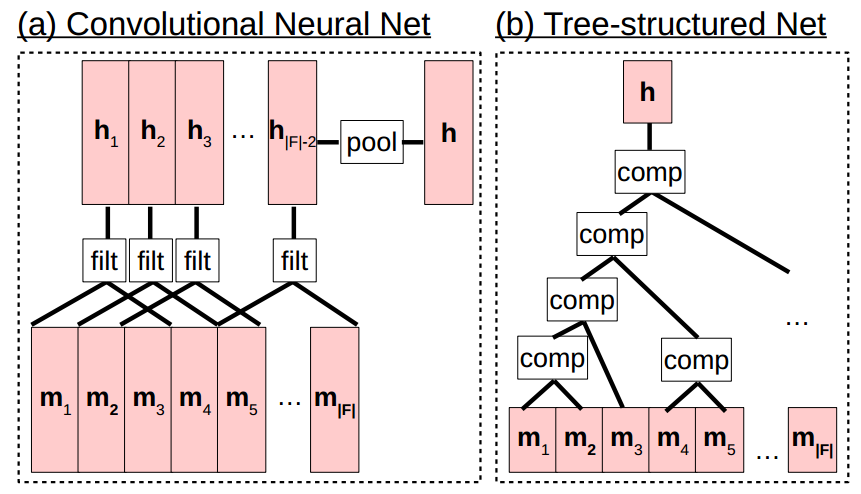
\includegraphics[width=0.7\textwidth]{fig25.png}
\caption{卷积神经网络和树结构神经网络的示例}
\label{fig:25}
\end{figure}

还有其他的一些解码方法,比简单地讲输入的句子看成是线性序列要复杂的多。例如,\textbf{卷积神经网络}模型(CNN;\cite{fukushima1988neocognitron,waibel1989phoneme,lecun1998gradient},图\ref{fig:25}(a))就是一类将空间或时间上局部片段的信息整合起来的模型。它们通常被应用在图像处理领域,但也已经被应用到语音处理任务和文本处理任务中来。虽然用来处理文本的基于CNN的模型有很多种(例如,\cite{kalchbrenner2014convolutional,lei2015molding,kalchbrenner2016neural}),在这里,我们例举\cite{kim2014convolutional}提出的一个模型。这个模型有长度为$w$的$n$个\textbf{过滤器filters},这些过滤器以$w$个词为窗口在输入上进行滑动。具体来说,给定一个宽度为$|F|$的词向量矩阵$M$,我们生成一个宽度为$|F|-w+1$的隐层矩阵$H$,这个矩阵的每一列等于:
\[
 \textbf{h}_t = W concat(\textbf{m}_t,\textbf{m}_{t+1},\cdots,\textbf{m}_{t+w-1})
\]
其中$W \in \mathbb{R}^{n \times w|m|}$是一个矩阵,其第$i$行表示过滤器$i$的参数,这个矩阵用来和$w$个连续的词的词向量相乘。如果$w=3$,我们可以这样理解,$\textbf{h}_1$是从$f_1^3$上提取的一个特征向量,$\textbf{h}_2$是从$f_2^4$上提取的一个特征向量,以此类推,直到句子结束。

最后,我们执行\textbf{池化(pooling)}操作,来将这个矩阵$H$(其宽度随着输入句子的长度而不同)转换成一个向量$\textbf{h}$(是一个固定长度的向量,因此可以用来进行后续的操作)。池化操作的一些例子,包括平均值、最大值,和$k$-最大值\cite{kalchbrenner2014convolutional}。

相比于RNN模型和其变种,CNN模型有一些优势和劣势:
\begin{itemize}
\item 好的方面,CNN模型提供了一种相对简单的方法,来挖掘句子中局部词序列的特征,并将这些特征积累到整个句子的层面。
\item 另一个好的方面,因为不需要在时间序列上多次向后传递梯度值,因此,CNN模型不会遭遇严重的梯度消失问题。
\item 作为不好的方面,CNN模型的标示性较弱,尤其是对于超过其过滤器宽度范围的复杂特征而言,CNN模型并不是一个特别自然的表示方法。
\end{itemize}

整体来说,我们发现CNN模型对于文本分类任务而言还是非常有效的,因为对于文本分类任务而言,捕获文本中最有指示性的特征才是非常重要的,而对文本的全局信息往往是次要的\cite{kim2014convolutional}。
当然,对于一些应用于端到端问题的CNN模型,也得到了一些很好的结果\cite{kalchbrenner2016neural}。

\subsubsection{树结构神经网络}
\begin{figure}[H]
\centering
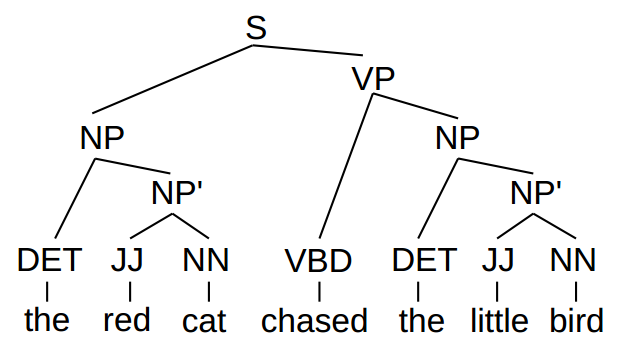
\includegraphics[width=0.6\textwidth]{fig26.png}
\caption{一个句法树样例,给出了句子的结构和短语类型}
\label{fig:26}
\end{figure}

最后,另一种在多个其他任务中经常被用到的编码器是\textbf{树结构神经网络}(\cite{pollack1990recursive,socher2011parsing}图\ref{fig:25}(b))。这些模型背后的基本思想是这样的,通过一些结构化的信息,比如句子的句法结构信息,来指导词与词之间信息的结合,在图\ref{fig:26}中给出了一个例子。
之所以这些结构化的信息在直观上是有用的,是因为每一个句法片段通常都是一个连贯的语义单位。因此,相比于CNN模型那样使用随机的子串序列的信息而言,使用这些连贯的语义单元上的向量来进行相关计算是更合理的。

举个例子来说,假设我们有图中所示的短句“the red cat chased the little bird”。这个例子中,使用句法树信息就能确保我们为语法词组对应的连贯语义单元的计算向量,这些语法词组比如这句话中的“chased”和“the little bird”,然后将这些词组的信息一个接一个的结合起来而获得更大的连贯词组的意义,比如“chased the little bird”。通过这样的操作,我们可以利用“语言是结构化的”这个事实,意思是,多个较小的短语片段通过常规的组合和转换过程可以得到更复杂的短语\cite{szabo2010compositionality}。通过从这种语言学上直观的角度来审视一个句子,我们希望这个信息能够帮助神经网络模型能从有限的训练语料中学习到更泛化的函数出来。

也许最简单的树结构神经网络是\cite{socher2011parsing}提出的\textbf{循环神经网络}模型。这个模型和标准的RNN模型非常相似,不同之处在于,和标准RNN模型按如下方式计算给定前一时刻$\textbf{h}_{t-1}$的情况下下一个隐层状态$\textbf{h}_t$不同:
\[
 \textbf{h}_t = tanh(W_{xh}\textbf{x}_t + W_{hh}\textbf{h}_{t-1} + \textbf{b}_h)
\]
我们在给定左孩子节点隐层状态$\textbf{h}_l$和右孩子节点隐层状态$\textbf{h}_r$的情况下计算父节点的隐层状态$\textbf{h}_p$,计算过程如下:
\[
 \textbf{h}_p = tanh(W_{xp}\textbf{x}_t + W_{lp}\textbf{h}_l + W_{rp}\textbf{h}_r + \textbf{b}_p)
\]
因此,树中的每个节点的表示可以通过一种从下到上的方式来计算得到。

和标准的RNN模型一样,这些循环神经网络也会遭遇梯度消失问题。为了解决梯度消失问题,有一种针对树结构的LSTM神经网络模型,叫做\textbf{tree LSTMs}\cite{tai2015improved}。
当然,还有很多种其他的树结构组合函数的建模方式,有兴趣的读者可以阅读\cite{socher2013parsing,dyer2015transition,dyer2016recurrent}。
还有一项有趣的研究\cite{li2015tree},通过研究NLP中的多个任务,来研究树结构能否对这些任务提供有用的信息。

\subsection{多个模型的融合}
在编码-解码模型或其他翻译模型中广泛使用的另一种方法,叫做\textbf{融合法}:通过结合多个独立训练的模型的预测结果来提升整体的预测结果准确率。
融合法背后的直观想法是这样的,不同的模型会犯不同的错误,当结果是正确的时候,相比于错误的时候而言,多个模型能够大概率的给出一致的预测结果。因此,如果我们将多个不同的模型融合起来,可以帮助平滑这些错误,更容易找到正确的答案。

融合编码-解码模型的第一步,就是独立地训练$N$个不同的模型$P_1(\cdot),P_2(\cdot),\cdots,P_N(\cdot)$,例如,在训练之前随机的初始化神经网络模型的参数。然后,在搜索解码过程中的每一个时刻,我们通过计算$N$个模型的概率结果的平均值来计算下一个词的概率分布:
\[
 P(e_t | F,e_1^{t-1}) = \frac{1}{N} \sum_{i=1}^{N} P_i(e_t | F,e_1^{t-1})
\]
这个概率分布将用于翻译假设的搜索过程中。

%\subsection{练习}

\section{注意力神经网络机器翻译}
在上一章节,我们介绍了一个简单的神经机器翻译模型,这个模型会用一个编码器将源语言句子编码为一个定长的向量。然而,在某种层面上,这种看问题的角度太过简单,通过引入\textbf{attention}这样一个强大的机制,我们可以解决这些难题。本章节将描述编码-解码架构所遇到的问题,以及如何通过attention机制来解决这些问题。

\subsection{编码-解码模型中特征表示的问题}
理论上,一个具有规模的并受过良好训练的编码-解码模型应该能够完美地完成机器翻译任务。正如在5.2节所介绍的那样,神经网络模型是通用的函数拟合器,意味着它们可以表示任何我们想要建模的函数,包括一个能够精准预测下一个词的分布概率$P(e_t | F,e_1^{t-1})$的预测函数。然而,在实际应用中,我们必须在有限的数据集上学习这些函数方程,在这个时候,最重要的是要有一个合适的\textbf{引导偏执inductive bias}--一个合适的模型架构从而使神经网络模型能够在合理规模的数据集上训练得到一个足够精度的概率模型。

让标准的编码-解码架构为难的事情主要有两个。第一个在前一章节已经讨论过:互为翻译的词条之间具有远距离的依赖关系。在前一章节中,我们通过逆向编码的策略部分的解决了这个问题并提高了训练效率,但仍旧没能解决很大一部分远距离依赖问题,并且很难保证我们能够训练出一个能够较好的处理这个问题的模型。

第二个让编码-解码架构为难的事情,是它尝试将不同长度的句子的信息存储到一个定长的隐层向量中。换句话说,即使我们期望机器翻译模型能够对长度为1到100个词的不同句子进行翻译,它任然是用相同的中间表示来存储这些输入句子的所有信息。如果我们的网络模型太小,那它就无法对我们行进行翻译的较长的句子的完整信息进行编码。另一方面,即使我们使用了一个足够处理输入中最长的句子的超大网络模型,在处理较短的句子时,这么大的模型又会成为灾难,因为需要使用大量的内存空间和计算开销。进一步地,因为这些网络模型会有较大的参数规模,在给定有限的训练数据时将很难对这些参数进行有效训练,很容易造成诸如过拟合等问题。

本节剩下的内容,将讨论一种更加自然的方式来用神经网络模型解决翻译问题:attention。

\subsection{注意力}
Attention机制背后的基本思想是这样的,我们不再尝试学习每一个句子的一个向量表示,而是将输入的句子中每一个词的向量表示都考虑进来,并在解码阶段的每一个时刻都来引用这些词的向量表示。因为可以引用的向量个数和输入句子中的词条个数相同,长句子会有多个向量而短句子会有较少的向量。作为结果,我们可以用更加有效的方式来表示输入的句子信息,从而解决前一节中提到的有效编码困难问题,即编码-解码模型遇到的无法对输入句子有效表示的问题。

首先,我们构造一系列的向量,我们将用这些向量来对不同长度的句子进行表示。为了做到这一点,我们为源语言句子中的每一个词计算一个向量表示,用一个RNN模型在两个方向上进行隐层状态向量计算:
\[
 \overrightarrow{\textbf{h}}_j^{(f)} = RNN(embed(f_j),\overrightarrow{\textbf{h}}_{j-1}^{(f)})
\]
\[
 \overleftarrow{\textbf{h}}_j^{(f)} = RNN(embed(f_j),\overleftarrow{\textbf{h}}_{j+1}^{(f)})
\]
然后,我们将两个向量$\overrightarrow{\textbf{h}}_j^{(f)}$和$\overleftarrow{\textbf{h}}_j^{(f)}$收尾相接而得到一个双向表示向量$\textbf{h}_j^{(f)}$:
\[
 \textbf{h}_j^{(f)} = [\overleftarrow{\textbf{h}}_j^{(f)};\overrightarrow{\textbf{h}}_j^{(f)}]
\]
进一步地,我们可以将不同时刻的向量拼接成一个矩阵:
\[
 H^{(f)} = concat_col(\textbf{h}_1^{(f)},\cdots,\textbf{h}_{|F|}^{(f)})
\]
这样,我们就得到了一个矩阵,该矩阵中的每一列,和输入句子中的每一个词相对应。

然而,我们现在遇到了一个难题。我们有一个矩阵$H^{(f)}$,其中包含不定个数个列向量,其个数随着源语言句子的长度而变化,但我们想用它来计算输出词汇的概率分布,而我们目前只知道如何在给定一个定长的向量作为输入时怎么计算这个概率分布。Attention机制的关键点在于,我们计算出一个向量$\textbf{$\alpha$}_t$,用这个向量来将矩阵$H$中的所有列向量加权平均成一个向量$\textbf{c}_t$:
\[
 \textbf{c}_t = H^{(f)} \textbf{$\alpha$}_t
\]
这个权值向量$\textbf{$\alpha$}_t$被称为\textbf{attention向量},其中元素一般符合这样的规则:元素值介于0到1之间且全部元素的和为1。

\begin{figure}[H]
\centering
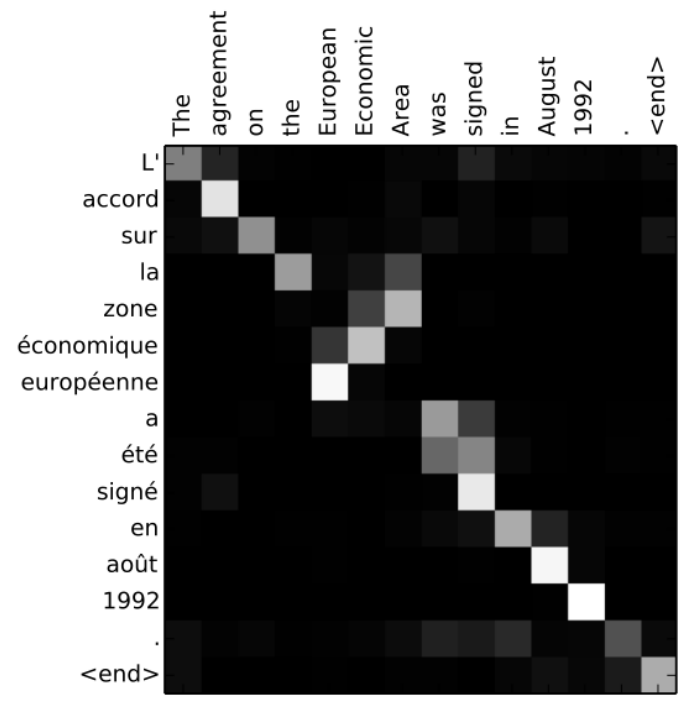
\includegraphics[width=0.7\textwidth]{fig27.png}
\caption{文献\cite{bahdanau2014neural}中给出的一个attention例子。源语言为英语,目标语言为法语,在生成某个目标词时Attention权重越高的地方,矩阵中相应方框中的灰度值越低}
\label{fig:27}
\end{figure}

Attention向量背后的基本思想是这样的,它会告诉我们在某一个特定的时刻模型对源语言句子中的某个词的“关注”程度。向量$\textbf{$\alpha$}_t$中的某个元素的值越大,则表示这个元素对应的源句词条在预测输出句子中的下一个词时具有更大的影响力。在图\ref{fig:27}中给出了一个样例,来说明Attention机制是如何在翻译过程中起作用的,我们可以看到,对齐向量中的元素数值和我们的直观感觉是大体上一致的。

\subsection{计算注意力得分}
那么下一个问题就变成“我们如何来计算得到这个向量$\textbf{$\alpha$}_t$?”了。
这个问题的答案在\textit{解码}RNN模型上,我们用解码RNN模型在生成输出序列时会跟踪当前的隐层状态。
和以前一样,解码器的隐层状态向量$\textbf{h}_t^{(e)}$也是一个定长的向量,这个向量表示前面已经生成的所有目标词序列$e_1^{t-1}$,其初始值为$\textbf{h}_0^{(e)} = \textbf{h}_{|F|+1}^{(f)}$。
换种表述方式的话,也就是说计算一个上文表示向量$\textbf{c}_t$,用它来表示在预测下一个目标词$e_t$时模型关注的源端上文信息,且其初始值为$\textbf{c}_0 = \textbf{0}$。

首先,我们基于解码过程中的前一时刻的词表示和上文向量来更新当前的隐层状态向量$\textbf{h}_t^{(e)}$:
\[
 \textbf{h}_t^{(e)} = enc([embed(e_{t-1});\textbf{c}_{t-1}],\textbf{h}_{t-1}^{(e)}).
\]

在这个向量$\textbf{h}_t^{(e)}$的基础上,我们计算\textbf{attention得分向量}$\textbf{$\alpha$}_t$,其中每一个元素的值等于:
\[
 \alpha_{i,j} = attn_score(\textbf{h}_j^{(f)},\textbf{h}_t^{(e)}).
\]
其中$attn_score(\cdot)$可以是任意的函数,其输入是两个向量,而输出时一个得分值,用来表示在翻译时刻$\textbf{h}_t^{(e)}$时我们对词编码向量$\textbf{h}_j^{(f)}$的关注程度。我们在8.4节末会介绍一些这个函数的例子。

然后我们用softmax函数,来对这个得分向量进行归一化,将其转换成一个正式的Attention向量:
\[
 \textbf{$\alpha$}_t = softmax(\textbf{$\alpha$}_t).
\]
然后我们把这个Attention向量作为一个权值向量,来将编码表示矩阵$H^{f}$中的列向量加权求和转换为上文向量表示$\textbf{c}_t$,作为当前翻译时刻的上文表示输入,如公式72所示那样。

现在,我们在$t$时刻有了上文向量$\textbf{c}_t$和隐层状态$\textbf{h}_t^{(e)}$,我们可以将它们传给后续的任务中使用。例如,我们可以将这两个向量首尾拼接起来,然后用softmax来计算下一个词的概率分布:
\[
 \textbf{p}_t^{(e)} = softmax(W_{hs}[\textbf{h}_t^{(e)};\textbf{c}_t] + b_s)
\]
这就意味着在计算输出词的概率分布时,每一个源语言句子中的词条的编码向量$\textbf{h}_j^{(f)}$都直接参与了这个最终概率分布的计算过程。
原先标准的编码-解码模型,只能在经过$|F|$步序列编码之后才能使用源语言句子中第一个词条所编码的信息,和它不同的是,现在源语言句子信息的编码可以通过公式72所示的上文向量的形式随时被使用到(以加权向量的形式使用)。

\begin{figure}[H]
\centering
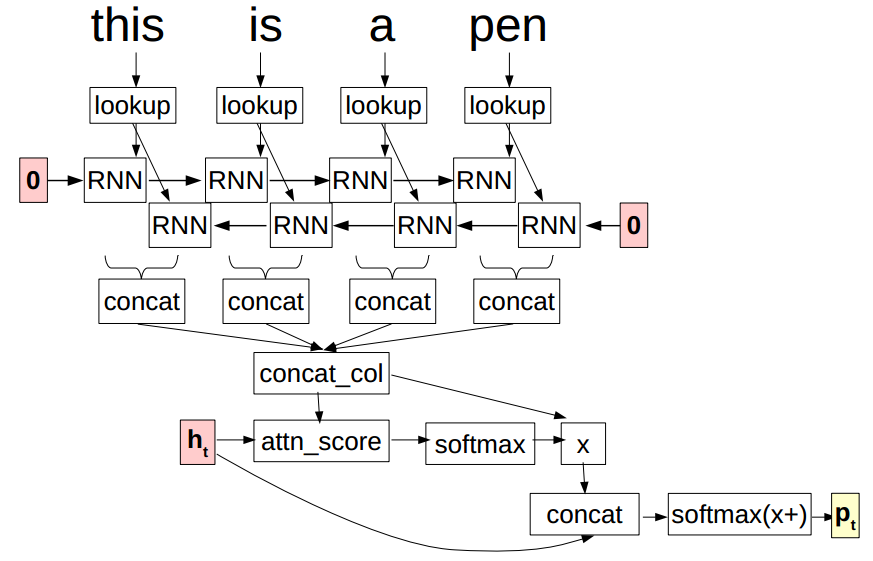
\includegraphics[width=0.7\textwidth]{fig28.png}
\caption{Attention的计算图示例}
\label{fig:28}
\end{figure}

在图\ref{fig:28}中给出了这个完整过程的示意图。

\subsection{计算注意力得分的不同方法}
如公式74所示,最后一块缺失的拼图,就是如何来计算这个Attention得分$\alpha_{t,j}$了。

文献\cite{luong2015effective}尝试了三种不同的Attention得分函数,它们都有各自的长处:
\begin{enumerate}
\item[] \textbf{点积函数:}这是最简单的一个得分函数,它只是简单地用点积来计算$\textbf{h}_t^{(e)}$和$\textbf{h}_j^{(f)}$之间的相似度:
\[
 attn_score(\textbf{h}_j^{(f)},\textbf{h}_t^{(e)}) := \textbf{h}_j^{(f)_{T}}\textbf{h}_t^{(e)}
\]
这个模型的好处在于它不会增加模型参数。然而,它还是有直观的缺陷的,因为这个方法会强制让输入和输出的编码在同一个特征空间(因为相似的$\textbf{h}_t^{(e)}$和$\textbf{h}_j^{(f)}$必定在空间上离得比较近,否则其点积结果不会很高)。还有一点值得一提,对源语言句子中所有词的编码向量的点积计算过程可以很快,只要我们用源语言上文编码拼接矩阵$H^{(f)}$与向量$\textbf{h}_t^{(e)}$的相乘来替换原有的Attention得分函数即可:
\[
 attn_score(H^{(f)}, \textbf{h}_t^{(e)}) := H_j^{(f)_T}\textbf{h}_t^{(e)}.
\]
将多个Attention得分计算操作合并到一起来计算,有助于我们得到更有效率的程序实现,尤其是在GPU上。下面的Attention得分函数也可以类似地进行快速计算。
\item[] \textbf{双线性函数:}对点积函数做一点点小的修改就可以得到更有表达能力的\textbf{双线性函数}。这个函数,通过在点积之前借助参数$W_a$进行一个线性变换操作,从而可以缓解简单的点积函数所遇到的限制,即要求源端和目标端的词向量必须在同一特征空间中的这一限制:
\[
 attn_score(\textbf{h}_j^{(f)},\textbf{h}_t^{(e)}) := \textbf{h}_j^{(f)_{T}}W_a\textbf{h}_t^{(e)}
\]
这样做有一个好处,因为$W_a$不是一个方矩阵,那么输入的两个向量的大小就可以不一致,因此就可以让编码器和解码器拥有不同大小的隐层状态向量。然而,它也会给模型引入相当规模($|\textbf{h}^{(f)}| \times |\textbf{h}^{(e)}|$)的参数,而且训练这么多参数也不太容易。
\item[] \textbf{多层感知机:}最后,我们也可以用一个多层感知机来计算Attention得分,文献\cite{bahdanau2014neural}就在它们最初的Attention机制实现过程中使用了这个方法:
\[
 attn_score(\textbf{h}_j^{(f)},\textbf{h}_t^{(e)}) := \textbf{w}_{a2}^{T}tanh(W_{a1}[\textbf{h}_t^{e};\textbf{h}_j^{(f)}]).
\]
其中,$W_{a1}$是多层感知机第一层的权重矩阵,$w_{a2}$是其第二层的权值向量。这个方法就比点积函数灵活许多,通常而言其参数规模要小于双线性函数,且一般都能得到一个好的结果。
\end{enumerate}

除了上面所讲的常见的标准方法之外,也有一些计算Attention得分的更加复杂的方法。例如,可以使用循环神经网络\cite{yang2016neural}、基于文档结构的树结构神经网络\cite{yang2016hierarchical}、卷积神经网络\cite{allamanis2016convolutional}、或者结构化的模型\cite{kim2017structured}来计算Attention得分。

\subsection{复制机制和未登录词替换}
除了能够提高翻译的精度之外,Attention机制还有另一个很好的副作用,它能让我们更容易的跟踪源语言中的某个(些)词被翻译成了翻译结果中的哪个(些)词条。这样一来有一个显而易见的后果,我们可以像图27那样画出一个直观图,从而方便我们进行错误分析。

Attention机制的另一个好处在于,能让我们以更优雅的方式来处理源语言端的未登录词,即使用\textbf{未登录词替换}操作\cite{luong2014addressing}。这个方法的思路很简单,每次解码器预测到下一个词条是个未登录词<UNK>时,我们就查找这个时刻Attention得分最高的那个源语言句子中的词条,然后输出这个源语言词条而不是输出<UNK>。
如果我们这么做了,至少用户可以看到哪些词条没有被翻译出来,这样总比看到这些词条被舍弃或者被替换为占位符要好得多。

如文献\cite{brown1993mathematics}中描述的那样,我们也经常看到用对齐模型来获取一个翻译词典,然后用这个翻译词典来进一步辅助未登录词的替换操作。
具体来说,不再是直接将源词条复制到输出中去,而是这样来进行替换操作:如果选择的源词条是$f$,我们输出一个翻译概率$P_{dict}(e|f)$最大的目标语言词条$e$。
这样一来,能够确保在翻译过程中,翻译词典中的词条能被翻译成其最佳的翻译候选词条。

\subsection{注意力上的直观先验}
因为Attention机制在神经网络机器翻译模型中如此重要,研究人员已经提出了很多用来提升Attention预测精度的方法,包括通过引入直观驱动的先验概率来提升Attention机制的准确率。文献\cite{cohn2016incorporating}提出了几种在模型训练过程中使用偏执信息的方法,来确保Attention权重符合我们对语言之间的对齐关系的直观理解。

引入的信息主要有这么几类,这些信息都是受到传统统计机器翻译系统中使用的对齐方法的影响,关于传统统计机器翻译系统中使用的对齐模型可以参考文献\cite{brown1993mathematics}的内容。这些对齐模型可以简单的总结为:
\begin{enumerate}
\item[] \textbf{位置偏执:}如果两个语言的语序很相似,那么词对齐结果更可能会是对角线型的。在图27中这种情况就很明显。可以通过加入Attention机制的先验概率来鼓励这种对角对齐行为,即让处在对角位置上的两个语言的词之间的Attention得分更高。
\item[] \textbf{马尔科夫假设:}在很多语言中,我们可以假设这样一个条件,如果目标语言中的两个词是连续出现的,那么他们对应的源语言词条也应该是连续出现的。例如,在图27中,对英语中的所有连续词对儿这都是成立的,除了“the,European”和“Area,was”之外。为了利用这种特性,可以引入这样一种先验知识,即它会鼓励局部转移上的Attention,而抑制两次Attention之间的远距离跳跃。有一个基于这样的假设但实现方式不同的模型,叫做\textbf{局部Attention}模型\cite{luong2015effective},用神经网络模型本身来选择要Attention的源语言句子中的片段。
\item[] \textbf{Fertility:}我们可以这样假设,即有些词条在另一个语言中的翻译结果的词个数是确定的。例如,英文单词“cats”会被翻译为法语中的两个词“les chats”。Fertility先验信息就能利用这个事实的好处,当某个词条对齐的词过少或者过多时都会受到模型的惩罚。实际上,一个未经很好训练而得到的神经网络机器翻译系统都有这样一些主要问题:一遍遍的重复翻译同一个词,漏掉某个词的翻译,这都是不符合fertility限制的情况。正因为此,已经有很多种方法尝试在模型中引入对覆盖度信息的利用了\cite{tu2016modeling,mi2016coverage},或者将其作为解码过程中的一个限制条件来使用\cite{wu2016google}。
\item[] \textbf{双语对称:}最后,我们期望模型中的对齐模型能做的这一点,在进行从$F$到$E$的翻译过程中对齐的那些词条,在进行从$E$到$F$的翻译时也要相互对齐。为做到这一点,我们可以并行的训练两个翻译模型(即两个方向的翻译模型),并要求两个方向上计算出来的对齐矩阵是相似的。
\end{enumerate}
文献\cite{cohn2016incorporating}通过对这些方法的实验,发现双语对称限制是这些方法中最有效的方法。

\subsection{扩展阅读}
在本小节,如果读者还想进一步优化Attention模型,我们在这里给出几个优化方向:
\begin{enumerate}
\item[] \textbf{硬Attention:}如公式75所示,标准的Attention机制只是利用多个上文信息的简单合并结果。也有一些硬Attention的方法,即作出一个0/1判别来确定对某个特定的上文是关注还是不关注,文献\cite{lei2016rationalizing}从模型可解释性的角度出发来使用了这种硬Attention方法,而文献\cite{yu2016online,gu2016learning}是从循序渐进的处理文本的角度出发来使用这个方法的。
\item[] \textbf{有指导的训练Attention:}此外,有时候我们有一些人工标注好的双语对齐数据。可以通过设计一个适当的损失函数,在这个训练数据上训练Attention模型,这个损失函数会在模型作出错误的对齐预测时给予惩罚\cite{mi2016supervised}。
\item[] \textbf{记忆输入的其他方式:}最后,除了Attention机制之外,还有其他的方法来使用相关的信息。文献\cite{wang2016memory}提出了一种使用\textbf{记忆神经网络}的方法,这个神经网络模型拥有一个独立的记忆单元,可以在模型处理的过程中在这个记忆单元中写入或者读取信息。
\end{enumerate}

%\subsection{练习}

\section{结论}
这篇综述的内容涵盖了神经网络机器翻译和端到端模型的基本知识。从$n$-gram语言模型开始到最后的Attention模型,我们循序渐进的一步步提升模型的复杂度,最终讲到了目前很多端到端模型所在应用任务的业界最高水平。

在此值得一提的是,这是一个非常活跃的研究领域,还有很多高级的研究主题超出了本篇综述的内容范围,但那些已经掌握了基础知识并希望学到更多知识的读者,也许会对这些高级研究内容感兴趣。

\begin{enumerate}
\item[] \textbf{处理大词表:}神经网络机器翻译模型的一大软肋,是当词表规模变大时,模型的翻译能力也会变差;很难在有限的训练数据上学到那些低频词之间的翻译关系,并且计算消耗也会成为瓶颈。处理这个问题的一个方法,是将词拆分成更小的单元,比如字符\cite{chung2016character}或者子串\cite{sennrich2015neural}等。也可以使用覆盖面很广的翻译词典等外部数据来解决这种低频词翻译难题\cite{arthur2016incorporating}。
\item[] \textbf{优化翻译质量:}本篇综述中讲述的模型,其训练过程是最大化给定源语言句子时的目标语言句子的似然概率值$P(E|F)$,但在实际应用中,我们更在乎的是翻译结果的准确性。已经有很多研究工作试图解决这种训练目标与实际应用目标之间存在差异的问题,他们的思路都是直接将准确率的提升作为训练目标函数来训练翻译模型。具体而言,包括这么几种方法:用当前模型生成的采样结果来优化参数使得翻译结果准确率提升\cite{ranzato2015sequence,shen2015minimum},通过优化参数从而提升模型的鲁棒性,即在生成过程中如果遇到某处错误的翻译结果也能保证之后的翻译结果不受这个错误的影响\cite{NIPS2015_5956,norouzi2016reward},尝试着防止解码器搜索过程中会生成的错误\cite{wiseman2016sequence}。
\item[] \textbf{多语种学习:}到此为止,我们都假设我们在训练一个两个语言$F$和$E$之间的翻译模型。然而在现实生活中,世界上有很多语言,一些研究结果指出,如果我们能使用所有这些语言的数据来同时训练模型,那模型的效果也会有提升\cite{firat2016multi,johnson2016google,ha2016toward}。当然也可以使用迁移学习的策略,在一对儿语言之间训练一个翻译模型,然后将其适应到其他的语言对儿上去\cite{zoph2016transfer}。
\item[] \textbf{其他应用:}类似的端到端模型已经被应用到很多任务中了,从对话系统\cite{vinyals2015neural,shang2015neural}到自动文摘\cite{rush2015neural}、语音识别\cite{chan2016listen}、语音合成\cite{van2016wavenet}、图像字幕生成\cite{karpathy2015deep,vinyals2015show}、图像生成\cite{gregor2015draw},等等。
\end{enumerate}

这些内容,仅仅是这个快速发展的领域中的一小部分研究方向,希望这篇综述能够给读者提供足够的工具,来解决自己遇到的问题,并将这些模型应用到自己感兴趣的任务中去。

\newpage

\begin{appendix}
\bibliographystyle{IEEEtran}
\bibliography{book}
\end{appendix}

\end{document}

